\documentclass[12pt]{article}

%======Fonts and Margins=====================================================================
\usepackage[utf8]{inputenc}
\usepackage[T1,T2A]{fontenc}
\usepackage[english,russian]{babel}
\usepackage{anyfontsize}

\usepackage{extsizes}
\usepackage[a4paper,
            left=33mm,
            right=10mm,
            top=15mm,
            bottom=20mm]{geometry}

            
\usepackage{setspace}
\usepackage{ragged2e}
\usepackage[skip=10pt plus1pt, indent=30pt]{parskip}
%===========================================================================================

%=======Graphics============================================================================
\usepackage{graphicx}
\usepackage{caption}
\captionsetup[table]{position=bottom}
\usepackage{subcaption}
\usepackage{color}
%===========================================================================================

%=======Other===============================================================================
\usepackage{longtable}
\usepackage{soul}
\usepackage{pdfpages}
\usepackage{fancyhdr}
\usepackage{sectsty}
\usepackage{verbatim}
\usepackage{tabularx}
\usepackage{stmaryrd}
\usepackage[style=numeric]{biblatex}
\usepackage{zref-totpages}
%===========================================================================================

%=======Сommands============================================================================
\newcommand{\anonsection}[1]{\section*{#1}\addcontentsline{toc}{section}{#1}}
%=======End Сommands========================================================================

%=======Listings============================================================================
\usepackage{listings}
\definecolor{gray}{rgb}{0.4,0.4,0.4}
\definecolor{darkblue}{rgb}{0.0,0.0,0.6}
\definecolor{cyan}{rgb}{0.0,0.6,0.6}

\lstset{
  basicstyle=\ttfamily,
  columns=fullflexible,
  showstringspaces=false,
  commentstyle=\color{gray}\upshape
}

\lstdefinelanguage{XML}
{
  morestring=[b]",
  morestring=[s]{>}{<},
  morecomment=[s]{<?}{?>},
  stringstyle=\color{black},
  identifierstyle=\color{darkblue},
  keywordstyle=\color{cyan},
  morekeywords={xmlns,version,type}% list your attributes here
}
%===========================================================================================


%======DOCUMENT START ======================================================================
\begin{document}

%======StartTitle Page======================================================================

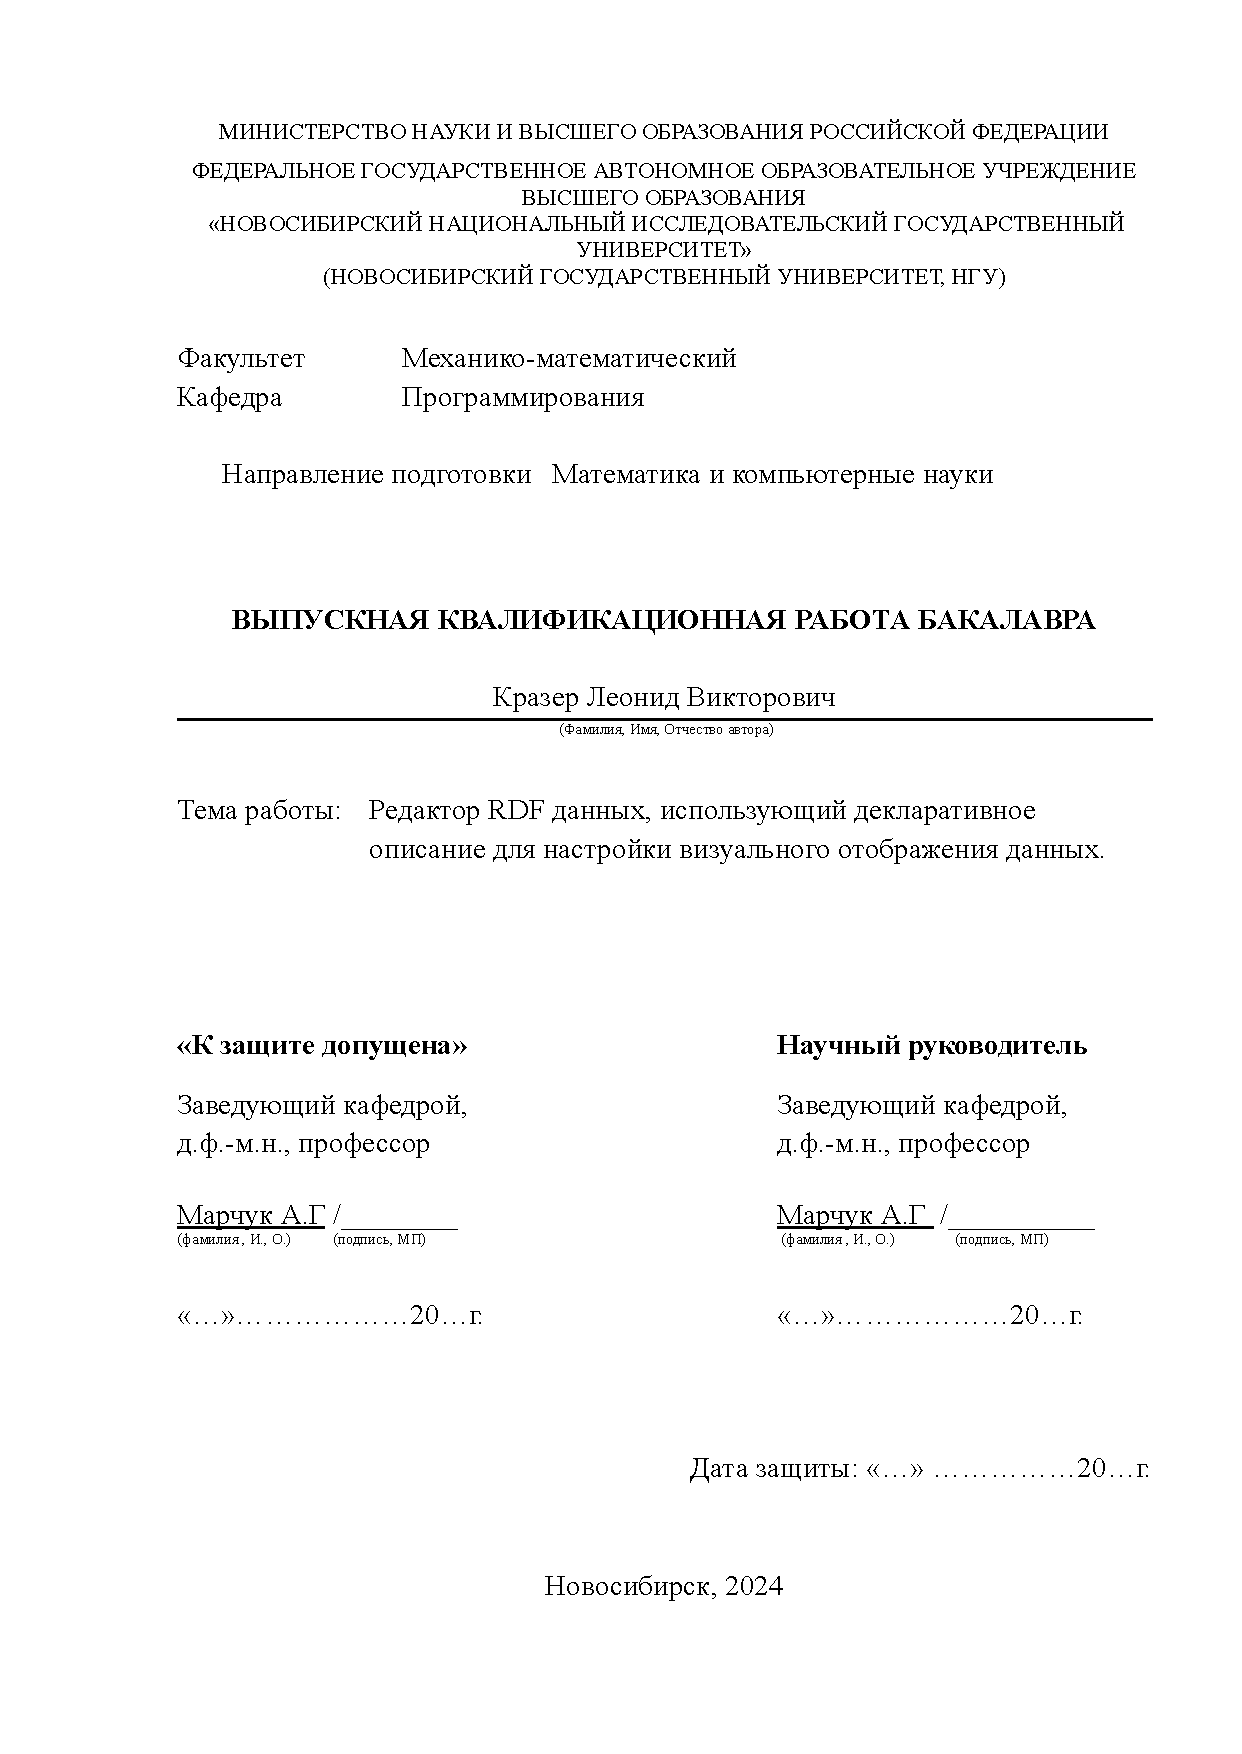
\includepdf[pages=-]{title_page.pdf}

%======EndTitle Page=======================================================================

%======Start Abstract======================================================================
\begin{center}
    {\anonsection{Реферат}}
\end{center}

До недавнего времени идея о информационной сети была для многих необъяснимой технологией, которую понимали только люди, которые активно работали с различными источниками информации, такие как IT администраторы, библиотекари, проектировщики информационных сетей и т.д. С того момента, как WWW стал широко распространен среди обычных людей, уже можно считать, что большинство немного знакомо с концепцией информационной сети, распространенной по всему земному шару. Главной идеей WWW является то, то есть основана она на открытом сообществе, вклад в которую может привнести любой человек, и в свою очередь любой человек может использовать данную информацию.\par

Однако чтобы сохранить консистентность и систематизировать всю информацию, которая находится в WWW, необходимы некоторые стандарты. Одним из таких стандартов, созданный W3C, является протокол RDF, который позволяет хранить информацию в структуре данных, называемой триплетом. Главным образом, данная работа посвящена созданию системы, предоставляющей удобные инструменты для анализа и редактирования RDF данных.\par

Работа содержит: $\ztotpages$ страниц, 3 главы, m рисунков, f источников.\par
Ключевые слова: Semantic Web, RDF, Клиент-Серверная архитектура
\pagebreak

%======End Abstract========================================================================

%======Содержание==========================================================================
\begin{center}
    {\anonsection{Содержание}}
\end{center}

\makeatletter
\@starttoc{toc}
\makeatother

\pagebreak
%======Конец Содержания====================================================================

%======Термины=============================================================================
\begin{center}
    {\anonsection{Терминология}}
\end{center}

\begin{center}
    \begin{tabular}{ | m{7cm} | m{7cm} | }
        \hline
        \textbf{Термин}                      & \textbf{Понятие}                                                                                                                                                      \\
        \hline
        WWW                                  & World Wide Web,  распределённая система, предоставляющая доступ к связанным между собой документам, расположенным на различных компьютерах                            \\
        \hline
        W3C                                  & World Wide Web Consortium, организация, разрабатывающая и внедряющая технологические стандарты для WWW                                                                \\
        \hline
        ПО                                   & Програмное обеспечение                                                                                                                                                \\
        \hline
        Semantic Web                         & Направление развития Всемирной паутины, целью которого является содержание данных вместе с сохранением их семантики                                                   \\
        \hline
        Фреймворк                            & Программная платформа, определяющая структуру программной системы, облегчающая создание других программ на своей базе                                                 \\
        \hline
        API                                  & Application Programming Interface - описание способов взаимодействия одной компьютерной программы с другими.                                                          \\
        \hline
        XML (eXtensible Markup Language)     & Расширяемый язык разметки. Позволяет дополнить разметку в соответствии с потребностями к конкретной области, будучи ограниченным лишь синтаксическими правилами языка \\
        \hline
        URI                                  & Последовательность символов, идентифицирующая абстрактный или физический ресурс                                                                                       \\
        \hline
        RDF (Resource Description Framework) & Разработанная W3C модель для представления данных                                                                                                                     \\
        \hline
        RDFS (RDF Schema)                    & Набор классов и свойств для модели представления знаний RDF, составляющий основу для описания онтологий с использованием расширенного RDF-словаря.                    \\
        \hline
        MVC/MVP/MVVM                         & Архитектурные шаблоны проектирования, предназначеные для разнесения логики и отображения в разные слои приложения.                                                    \\
        \hline
    \end{tabular}
\end{center}

\pagebreak

\begin{center}
    \begin{tabular}{ | m{7cm} | m{7cm} | }
        \hline
        \textbf{Термин}                                  & \textbf{Понятие}                                                                                                                                 \\
        \hline
        XAML (eXtensible Application Markup Language)    & Расширяемый язык разметки для приложений основанный на XML, используемый для декларативного программирования интерфейса приложений.              \\
        \hline
        DI/Dependency Injection (Внедрение зависимостей) & Шаблон проектирования, при котором поля объекта задаются внешней сущностью                                                                       \\
        \hline
        DI Контейнер                                     & Одна из реализаций паттерна DI, которая позволяет автоматизировать множество задач, включая компоновку объектов и управление их жизненным циклом \\
        \hline
        REST (REpresentational State Transfer)           & Архитектурный стиль взаимодействия компонентов распределённого приложения в сети                                                                 \\
        \hline
        Система управления версиями                      & Программное обеспечение для облегчения работы с изменяющейся информацией.                                                                        \\
        \hline
    \end{tabular}
\end{center}

\pagebreak
%======Конец Термины=======================================================================

%======Введение============================================================================
\begin{center}
    {\anonsection{Введение}}
\end{center}

WWW существует уже очень долгое время, и за это время в ней уже накопился огромный багаж знаний и различной информации. И она с каждым годом продолжает расширяться благодаря поддержке сообщества по всему миру. И на данный момент она представляет из себя множество фактов, которые дополняют, расширяют и которые при этом довольно часто противоречат друг другу. И тем не менее, для людей, которые готовы потратить свое время и силы, это не является преградой. Но все же, информационной сети не хватает таких качеств как структуризованность и консистентность, из-за чего она ощущается очень плоской. \par

Эта проблема возникает по той причине, что WWW связана на уровне представления (веб страниц), с помощью, например, гиперссылок[1]. Чтобы решить данную проблему, нужно рассматривать информационную сеть на уровне данных. В таком случае, информация должна быть не часть веб приложения, а частью самой информационной сети, чтобы любые другие приложения могли лекго получить доступ к этим данным.

Отсюда возникла инициатива по созданию семантической паутины, главным инициатором который стал Tim Berners-Lee, член W3C, чье видение заключалось в том, чтобы создать гибкую, само-адаптируемую и легко встраемую информационную сеть, которая предлагала пользователям более богатый опыт взаимодействия.\par

W3C разработал определенные инструменты и стандарты, чтобы развивать технологию Semantic Web, и которые на данный момент уже доступны. Наиболее важными из них в рамках этой работы являются способы хранения данных, пригодные для машинной обработки, основой которых является стандарт RDF, и различные схемы, с помощью которых можно описывать некоторые метаданные вокруг этих самых данных[2].\par

Среди людей, которые занимаются анализом данным или смежными вещами, может возникнуть необходимость в работе с структурами данных, основанных на стандарте RDF. И довольно часто эти данные имеют большой объём, а учитывая их формат, больше предназначенный для машинной обработки, чем для человека, время поиска и редактирования их может доставить пользователю множество трудностей.

В итоге цель работы можно сформулировать следующим образом: исследовать и, самое главное, разработать программное обеспечение, используя клиент-серверную архитектуру, которое позволило бы пользователю удобно с ними работать.\par

Основные задачи, которые будут выполнены в работе:
\begin{enumerate}
    \item Рассмотреть различные способы отображения RDF данных
    \item Разработать клиентскую часть приложения
          \begin{itemize}
              \item Построить модель данных для отображения в представление
              \item Реализовать логику отображения и редактирования данных
              \item Разработать пользовательский интерфейс
          \end{itemize}
    \item Разработать серверную часть приложения
          \begin{itemize}
              \item Исследовать различные базы данных
              \item Создать протокол взаимодействия сервера с клиентом
              \item Реализовать логику работы серверной части
          \end{itemize}
\end{enumerate}

В результате работы ожидается создание клиент-серверного приложения, упрощающего работу с RDF данными, которое предоставит удобное для восприятия представление данных и добавит интерактивные элементы в это представление, посредством создания различных режимов отображения, а также благодаря серверной части приложения у пользователя будет возможность работы с большими данными с любым устройством, при этом не имея необходимость хранить большой объем информации на своем физическом носителе.

\pagebreak
%======Конец Введения======================================================================

\sectionfont{\bfseries\Large}
\subsectionfont{\RaggedRight}
%======Предметная область==================================================================
\begin{center}
    {\section{Предметная область}}
\end{center}

\subsection{Модель задачи}
Предметной областью работы является инструменты для работы c Semantic Web, в частности стандарт хранения семантических данных Resource \\ Description Framework (RDF)[3] и стандарты описания онтологий, то есть метаданных об этих RDF данных. Ниже приведены ключевые особенности и понятия, которые регламентируют эти стандарты:\par

\subsubsection{Представление RDF стандарта}

\qquad Формат RDF был создан для того, чтобы можно было создавать утверждения о ресурсах в таком виде, который был бы пригоден для машинной обработки. Утверждение, высказываемое о ресурсе, имеет вид «субъект — предикат — объект» и называется триплетом. А RDF файл это соответственно множество таких триплетов.\par

Пусть есть некоторый субъект в виде участия в некотором мероприятия, у которого существует описание, участник и организация, в которой оно проходило. В этом примере субъектом является некоторое описание участия в организации, которое можно идентифицировать как participation1, участника в нем можно найти по идентификатору person1, и само участие проходило в организации под идентификатором conference1. В деталях просто указано "participate".

На рис. \ref{fig:eric} изображено понятное для человека представление конкретного участия, на рис. \ref{lst:eric} записано тоже самое в виде стандарта RDF в XML реализации. Пока что непонятно, что написано в последнем, поэтому следует разобраться как все устроено в RDF стандарте.\par

\begin{figure}[!b]
    \centering
    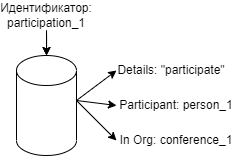
\includegraphics{_images/eric.png}
    \caption{Человеко-понимаемый формат}
    \label{fig:eric}
\end{figure}

\pagebreak

\begin{figure}
    \begin{lstlisting}[language=XML]
        <?xml version="1.0" encoding="utf-8"?>
        <rdf:RDF xmlns:rdf=".../22-rdf-syntax-ns#">
        <participation rdf:about="participation_1">
            <details>participate</details>
            <participant rdf:resource="person_1" />
            <in-org rdf:resource="conference_1" />
        </participation>
        </rdf:RDF>
    \end{lstlisting}
    \caption{RDF Представление}
    \label{lst:eric}
\end{figure}

\subsubsection{Реализации RDF стандарта}
\qquad На данный момент есть множество различных реализаций стандарта RDF данных. Все они так или иначе отличаются синтаксисом объявления утверждений. Из них наиболее популярны следующие форматы:\par

\paragraph{RDF / XML} [4, 9] (рис. \ref{lst:xml_rdf}) - самый старый из существующих форматов представления RDF данных. Главным плюсом является то, что он построен на базе спецификации XML документа, чтение и запись которого довольно удобна из-за большого количества библиотек, работающих с XML. Большой проблемой является его многословный синтаксис, из чего также следует тот факт, что файл в таком формате может занимать намного больше места чем при других форматах сериализации RDF.\par

\begin{figure}[!ht]
    \begin{lstlisting}[language=XML]
    <rdf:RDF xmlns:rdf=".../22-rdf-syntax-ns#"> 
        <participation rdf:about="participation_1">
            <details>participate</details>
            <participant rdf:resource="person_1" />
            <in-org rdf:resource="conference_1" />
        </participation>
    </rdf:RDF>
    \end{lstlisting}
    \caption{XML реализация RDF}
    \label{lst:xml_rdf}
\end{figure}

\paragraph{Notation3 (N3)} [5] (рис. \ref{lst:n3_rdf}) - формат сериализации данных, предложенный Tim-Berners Lee, в противовес RDF/XML. Имеет большое количество дополнительной функциональности, из-за чего сериализация данного формата может оказаться довольно трудоемкой.

\begin{figure}[!ht]
    \begin{lstlisting}[language=XML]
        @prefix rdf:     <.../22-rdf-syntax-ns#> .

        participation_1 details "participate".
        participation_1 participant person_1 .
        participation_1 in-org conference_1  .
    \end{lstlisting}
    \caption{N3 реализация RDF}
    \label{lst:n3_rdf}
\end{figure}

\pagebreak

\paragraph{Turtle} [6] (рис. \ref{lst:ttl_rdf}) - формат сериализации данных, являющийся подмножеством Notation3. В нем отсутствует множество особенностей Notation3, что делает его более быстрым в плане сериализации, но при этом оставаясь относительно легко воспринимаемым для человека.

\begin{figure}[!ht]
    \begin{lstlisting}[language=XML]
        @prefix rdf:     <.../22-rdf-syntax-ns#> .

        participation_1 details "participate".
        participation_1 participant person_1 .
        participation_1 in-org conference_1  .
    \end{lstlisting}
    \caption{Turtle реализация RDF}
    \label{lst:ttl_rdf}
\end{figure}

\subsubsection{Структура RDF триплета}
\hphantom{text}
\begin{figure}[!ht]
    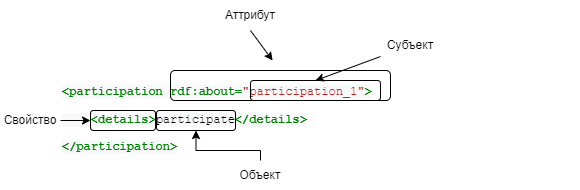
\includegraphics[width=1\textwidth]{_images/rdf_eric_razbor.png}
    \caption{Структура триплета}
    \label{fig:rdf_deconstruction}
\end{figure}

Как говорилось ранее, RDF тройки состоят из субъекта, предиката и объекта. В данном случае (рис. \ref{fig:eric}) говорится о том, что субъект под именем participation1 обладает свойством details, которое равно строковому значение <<participate>>. Как можно заметить, тут появилась такая сущность как атрибут, которая существует в контексте RDF/XML формата. Атрибут rdf:about указывает на то, какой уникальный идентификатор у субъекта. У субъекта вместе с этим атрибутом может быть и другие. В данном случае (рис. \ref{fig:rdf_deconstruction}) имеется уникально идентифицированый субъект и свойство, а сам объект уже нет, и в таком случае они называются литералами. У субъекта могут быть в качестве объекта другие уникально идентифицированные сущности. Для этого используется атрибут rdf:resource. Причем эта сама сущность может содержать в себе значение, так и не содержать, где в таком случае она называется пустым узлом.

\subsection{Онтологии}
\qquad Онтология[1] - это механизм, который позволяет определяеть термины, используемые для описания и представления определенной области знаний. Онтологии используются людьми, базами данных и приложениями, которым необходимо обмениваться информацией о конкретной предметной области, как например, в медицине, управлении финансами и т. д. Онтологии включают в себя пригодные для использования компьютером определения основных понятий и связей между ними, тем самым делая их многократно используемыми, а также дает им возможность встраиваться в другие возможножные области знаний. Эти области знаний могут быть простыми, как например иерархии и таксономии, так и довольно сложными, как например математические теоремы.

Сами онтологии можно структуризовать следующим образом:
\begin{enumerate}
    \item Классы в интересующей области знаний.
    \item Отношения между этими классами.
    \item Свойства, которые описывают конкретный класс.
\end{enumerate}

Для того, чтобы эти онтологии можно было реализовывать, W3C разработал такие стандарты как RDF, о котором было рассказано выше, RDF Schema и OWL.

\subsubsection{RDF Schema}
\qquad Как было сказано ранее, RDF определяет простую модель для описания объекта, который рассматривается в качестве ресурса, а также как связи между ресурсами в терминах идентифицируемых свойств и значений. RDF Schema (RDFS) служит для задачи структуризации предметной области, а именно типов и свойств, то есть предоставляет базовую систему типов.\par

Как уже было указано, RDFS определяется в терминах базовой информационной модели RDF – структуры графа, который описывает ресурсы и свойства. Все RDF схемы используют некоторую базовую структуру: они описывают классы ресурсов и типы связей между ресурсами. Эта общность разрешает использовать другие схемы для описания разных областей знаний, оставаясь также пригодными для машинной обработки, и отвечать требованиям по созданию метаданных, в которых утверждения могут быть получены из множества разнородных децентрализованных схем, созданных различными сообществами по разным принципам и разными методами.\par

Разберем наиболее важные понятия и свойства, которые предоставляет RDFS:

\paragraph{Class}
Позволяет идентифицировать некоторое множество, куда могут входить сущности.

\begin{lstlisting}[language=XML]
<Class rdf:about="http://fogid.net/o/sys-obj" />
\end{lstlisting}

\paragraph{SubClassOf}
Свойство, которое позволяет установить тот факт, что любой объект производного типа является также объектом базового типа, а также имеет все те свойства, которые есть у базового типа

\begin{lstlisting}[language=XML]
<Class rdf:about="http://fogid.net/o/org-sys">
    <SubClassOf rdf:resource="http://fogid.net/o/sys-obj"/>
</Class>
\end{lstlisting}

\paragraph{domain и range}
Когда мы описываем использование терминов в наших данных, мы также хотим представить, как свойство используется относительно определенных классов. В частности, мы можем захотеть сказать что при использовании свойства domain субъект принадлежит к определенному классу, а объект - из какого-то другого типа, указанного в свойстве range. Так существует возможность указывать какие свойства и их тип значения может содержать типизированная сущность.

\begin{lstlisting}[language=XML]
<DatatypeProperty rdf:about="http://fogid.net/o/name">
    <domain rdf:resource="http://fogid.net/o/sys-obj"/>
    <range rdf:resource="http://fogid.net/o/text"/>
</DatatypeProperty>
\end{lstlisting}

\paragraph{label}
Данное свойство предоставляет читаемое название для некоторого типа.

\begin{lstlisting}[language=XML]
<Class rdf:about="http://fogid.net/o/person">
    <label xml:lang="en">Person</label>
    <SubClassOf rdf:resource="http://fogid.net/o/sys-obj"/>
</Class>
\end{lstlisting}

\subsubsection{Web Ontology Language}
\qquad Следующим шагом в развитии технологии Semantic Web стал язык Web Ontology Language (OWL)[8], который выходит за пределы базовых конструкций, представленных в RDF Schema. Новые конструкции в OWL, такие как отношения между классами, мощность  и эквивалентность множеств и большое количество новых способов описания свойств и типов, позволяет описывать более точно онтологии.

Основная особенность OWL является то, что он следует формальной логике. Благодаря этому существуют механизмы, позволяющие из заданных терминов выводить совершенно новые термины.

OWL нельзя назвать конкретным языком, так как это общее название для таких языков как:
\begin{enumerate}
    \item OWL Lite - самый простой язык, который позволяет строить иерархии и накладывать простые ограничения на классы и свойства.
    \item OWL DL - содержит в себе все конструкции, представленные в OWL. На некоторые конструкции OWL накладываются определенные ограничения по применимости, но в замен существует гарантия того, вывод новых терминов будет выполнен за конечное время.
    \item OWL Full - предоставляет полный набор конструкций OWL, но остутствует гарантия что вывод новых терминов будет выполнен законечное время, если вообще будет выполнен.
\end{enumerate}

\subsubsection{Применимость онтологии в данной работе}
\qquad Онтологии очень важны для приложений, в которых нужно взаимодействовать с информацией, полученных из разных источников. Хотя XML или JSON[10] достаточны для обмена данными между сторонами, заранее согласовавшими определения, отсутствие в них семантики не позволяет машинам надежно выполнять эту задачу, учитывая новые словари XML. Один и тот же термин может использоваться с (иногда едва уловимым) разным значением в разных контекстах, и разные термины могут использоваться для элементов, имеющих одинаковое значение. Языки и стандарты описания онтологий позволяют решить эту проблему, связывая типизацию классов с идентификаторами. С помощью онтологий можно определять классы, которые могут иметь множество подклассов и суперклассов, а также определять свойства, которые могут иметь подсвойства, у которых есть зафиксированные домены и диапазоны. Более подробно о том, как применяются онтологии будет рассказано в главах \ref{sect:tables} и \ref{sect:Rdf_Vis}

\subsection{Используемые данные}
\qquad В рамках этой работы используется RDF база данных, описывающая некоторые факты о проведении Летней Школы Юных Программистов, а также онтология, с помощью которой описаны эти факты и связи между ними.

Базовыми классами в построении иерархии объектов служат такие классы как Sys-Obj -- Системный объект и Entity -- Сущность (рис. \ref{fig:ent_sys_obj}). Любая сущность в рамках этой онтологии может иметь комментарий, а также некоторый временной промежуток существования. У сущности типа Sys-Obj, помимо унаследованных свойств Entity также есть имя и описание.

\begin{figure}[!ht]
    \centering
    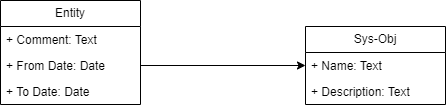
\includegraphics[width=0.6\textwidth]{_images/base_sch_onto.png}
    \caption{Классы Entity и Sys-Obj}
    \label{fig:ent_sys_obj}
\end{figure}

Поверх первого класса строится иерархия системных объектов (рис. \ref{fig:sys_obj_hier}). Среди них можно выделить Person - представление персоны, Org-Sys - модель некоторой организационной системы, Document - некоторая информация в виде текста, изображения или других медиа форматах, Geo-Sys - сущность, предоставляющая местоположение объекта и Collection - хранилище для системных объектов.

\begin{figure}[!ht]
    \centering
    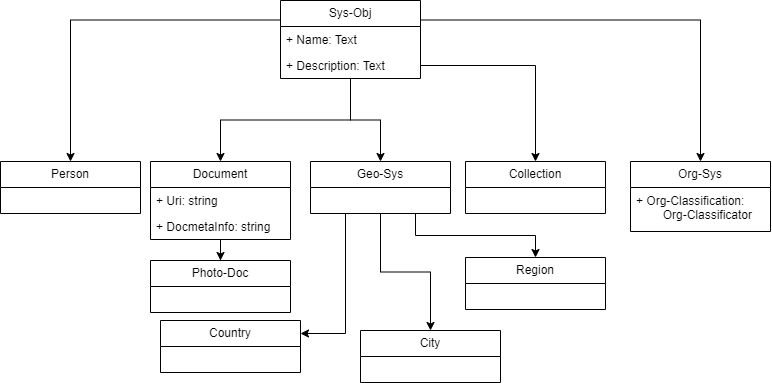
\includegraphics[width=0.9\textwidth]{_images/sys_obj_all.png}
    \caption{Иерархия системных объектов}
    \label{fig:sys_obj_hier}
\end{figure}

\pagebreak

Иерархия сущностей (рис. \ref{fig:ent_obj_hier}) состоит из объектов Participation, описывающего участие в событии и ключевую роль в этом событии, Location, который указывает место системного объекта, а также сущностей Reflection, Collection-Member, позволяющих создавать связи между системными объектами и документами, в которых они описаны.

\begin{figure}[!ht]
    \centering
    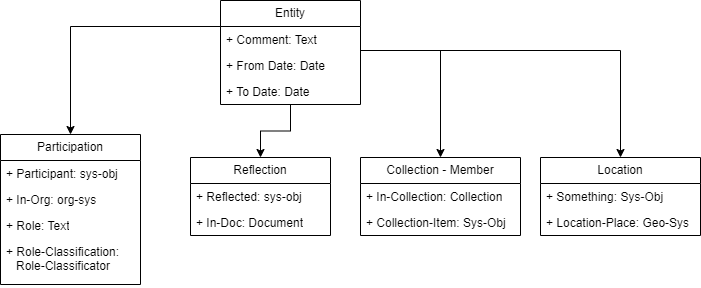
\includegraphics[width=0.9\textwidth]{_images/ent_all.png}
    \caption{Иерархия сущностей}
    \label{fig:ent_obj_hier}
\end{figure}

Также данная онтология предоставляет новые свойства и классы, такие как:

\paragraph{EnumerationType} Предоставляет ограниченное множество значений, имеющих общий тип.

\begin{lstlisting}[language=XML]
<EnumerationType rdf:about="http://fogid.net/o/org-classificator">
    <state value="team" xml:lang="en">group</state>
    <state value="arrangement" xml:lang="en">event</state>
    <state value="club" xml:lang="en">club</state>
</EnumerationType>
\end{lstlisting}

\paragraph{ObjectProperty} Является подтипом свойства, которое ограничивает свойство range объектными типами
\begin{lstlisting}[language=XML]
<ObjectProperty rdf:about="http://fogid.net/o/father">
    <label xml:lang="en">father</label>
    <inverse-label xml:lang="en">child</inverse-label>
    <domain rdf:resource="http://fogid.net/o/person"/>
    <range rdf:resource="http://fogid.net/o/person"/>
</ObjectProperty>
\end{lstlisting}

\paragraph{DatatypeProperty} Является подтипом свойства, которое ограничивает свойство range литеральными типами
\begin{lstlisting}[language=XML]
<DatatypeProperty rdf:about="http://fogid.net/o/org-category">
    <label xml:lang="en">organization form</label>
    <domain rdf:resource="http://fogid.net/o/org-sys"/>
    <range rdf:resource="http://fogid.net/o/text"/>
</DatatypeProperty>
\end{lstlisting}

\paragraph{inverse-label} Данное свойство предоставляет читаемое название для обратной ссылки (глава \ref{sect:inv_link})
\begin{lstlisting}[language=XML]
<ObjectProperty rdf:about="http://fogid.net/o/collection-item">
    <label xml:lang="en">contains</label>
    <inverse-label xml:lang="en">collection's element</inverse-label>
    <domain rdf:resource="http://fogid.net/o/collection-member"/>
    <range rdf:resource="http://fogid.net/o/sys-obj"/>
</ObjectProperty>
\end{lstlisting}

\subsection{Дополнительные данные}
Чтобы показать преимущества работы с клиент-серверным приложением, в качестве примера используется дамп словаря Medical Subject Headings (MeSH)[11], индексирующий журнальные статьи и книги по естественным наукам. На 2017 год (время создания дампа), он содержит более 14 млн. предметных рубрик, большинство из которых сопровождаются кратким описанием или определением, ссылками на другие рубрики, а также списком синонимов или схожих терминов. Итоговый размер файла дампа составляет 1.8 Гб., используемый стандарт сериализации RDF - Turtle.

\subsection{Визуализация RDF данных}
\qquad На текущий момент существуют инструменты, которые позволяют отображать RDF данные, в особенности связи между различными индивидуальными сущностями, записанными в этом формате. Однако для этого эти инструменты прибегают к тяжелым графическим представлениям, что во-первых является ресурсозатратным, а во вторых отображение больших объемов данных приводит к тому, что невозможно разместить все узлы таким образом, чтобы можно было визуально изучить структуру графа.

Соответственно, нужно найти способ, чтобы можно было не используя тяжелые графические представления, ясно и компактно выразить большое количество данных, записанных в формате RDF. Подробнее о предложенных методах будет рассказано в главе \ref{sect:Rdf_Vis}

\subsection{Вывод по первой главе}
\qquad В этой главе дано краткое описание предметной области проекта, а именно: стандарт и реализация RDF спецификации, пространства имен, часть RDFS спецификации. Также были в данной главе рассмотрены основные источники данных, с которыми велась работа.

\pagebreak
%======Конец Предметная область============================================================

%======Архитектура и алгоритмы=============================================================
\begin{center}
    {\section{Архитектура и алгоритмы}}
\end{center}

Существует множество архитектурных подходов по созданию пользовательских приложений. В рамках этой работы выбрана клиент-серверная архитектура (рис. \ref{fig:client_server_arch}), так как она позволяет отделить логику от данных. Благодаря этому мы можем не требовать от пользователя хранить эти данные у себя на компьютере, а также поддерживать работу нескольких пользователей над одним источником данных.

\begin{figure}[!ht]
    \centering
    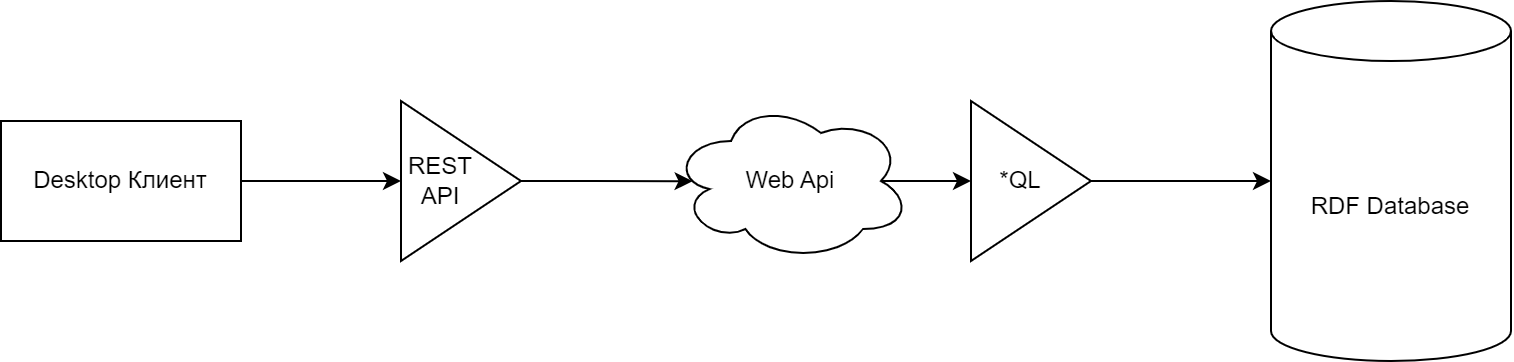
\includegraphics[width=1\textwidth]{_images/architecture.png}
    \caption{Клиент-серверная архитектура}
    \label{fig:client_server_arch}
\end{figure}

\subsection{Клиентская часть приложения}
\qquad Клиентская часть сделана с помощью фреймворка WPF[12], инструмента для создания пользовательских приложений для Windows платформ. Выбор этого фреймворка обусловлен тем, что он имеет намного больше возможностей для построения больших пользовательских приложений, а также на данный момент он имеет огромную пользовательскую поддержку в плане библиотек и других фреймворков, почти не содержит багов и недоработок, и в целом быстрее чем браузерные аналоги[TODO], так как используется высокопроизводительная платформа Microsoft .NET вместе с аппаратным ускорением на базе графического API DirectX[TODO] .\par

\subsubsection{WPF}
\qquad Фреймворк WPF базируется на архитектурном шаблоне MVVM[13] (рис. \ref{fig:mvvm}). MVVM удобно использовать вместо классического MVC[14] и ему подобных в тех случаях, когда в платформе, на которой ведётся разработка, есть «связывание данных» (data binding)[3]. В шаблонах проектирования MVC/MVP[15] изменения в пользовательском интерфейсе не влияют непосредственно на Mодель, а предварительно идут через Контроллер (англ. Controller) или Представитель (англ. Presenter). В таких технологиях как WPF есть концепция «связывания данных», позволяющая связывать данные с визуальными элементами в обе стороны. Следовательно, при использовании этой концепции применение шаблона MVC становится крайне неудобным из-за того, что привязка данных к представлению напрямую не укладывается в концепцию MVC/MVP.\par

\begin{figure}[!ht]
    \centering
    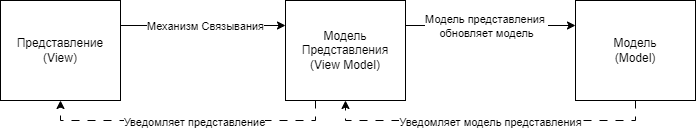
\includegraphics[width=1\textwidth]{_images/mvvm.png}
    \caption{Шаблон проектирования MVVM}
    \label{fig:mvvm}
\end{figure}

\begin{itemize}
    \item Модель (англ. Model) представляет собой логику работы с данными и описание фундаментальных данных, необходимых для работы приложения.

    \item Представление (англ. View) — графический интерфейс (окна, списки, кнопки и т. п.). Выступает подписчиком на событие изменения значений свойств или команд, предоставляемых View Model. В случае, если в View Model изменилось какое-либо свойство, то она оповещает всех подписчиков об этом, и View, в свою очередь, запрашивает обновлённое значение свойства из View Model. В случае, если пользователь воздействует на какой-либо элемент View, то вызывает соответствующую команду, предоставленную View Model.

    \item Модель Представления (англ. View Model) — с одной стороны, абстракция View, а с другой — обёртка данных из Model, подлежащиx связыванию. То есть, она содержит Model, преобразованную к View, а также команды, которыми может пользоваться View, чтобы влиять на Model.
\end{itemize}

\subsubsection{WPF Prism}
\qquad WPF Prism[16] является фреймворком для WPF, который собирает и реализует все лучшие практики, наработанные многими командами, работающие не только с самим WPF, но и другими MVVM фреймворками, такими как AngularJS, Vue.js и другие. Главные его особенности это предоставление инструментов для создания сложных многомодальных приложений, разделение этого приложения на различные контексты (модули), а также удобный механизм внедрения зависимостей. Так как разрабатываемое приложения соответствует всем этим пунктам, было решено использовать данную технологию.\par

\subsubsection{Модель данных на уровне клиента}
\qquad Так как формат RDF подразумевает под собой, что можно его представить в виде графа, то было решено выразить модель данных именно в таком виде, а не в форме множества троек субъект-предикат-объект (рис. \ref{fig:record}).

\begin{figure}[!ht]
    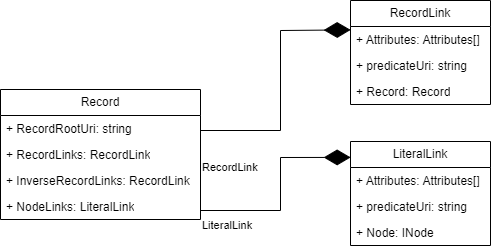
\includegraphics[width=1\textwidth]{_images/record_literal.png}
    \caption{Модель RDF записи}
    \label{fig:record}
\end{figure}

\subsubsection{Обратные ссылки} \label{sect:inv_link}
\qquad Хоть RDF формат не предполагает существование обратных ссылок (рис. \ref{fig:inverse_link}), так как он по идее строит ориентированный граф, их наличие помогает во многих ситуациях. Это может помочь в быстром нахождении всех записей, которую ссылаются на данную, а также в таких инструментах как удаление некоторой записи. Если бы обратных ссылок не было, в таком случае бы пришлось проверять у каждой вершины, содержит ли она ссылку на удаленную вершину, что заняло бы O(n $\times$ m) времени, где n - количество вершин, m $\ll$ n - количество связей. При использовании обратных ссылок, мы можем это сделать за O(m $\times$ m).

\begin{figure}[!ht]
    \centering
    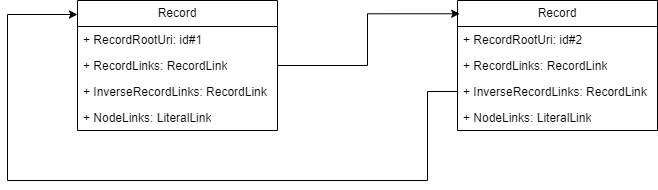
\includegraphics[width=0.8\textwidth]{_images/inverse_link.png}
    \caption{Структура записи с обратными ссылками}
    \label{fig:inverse_link}
\end{figure}

\subsection{Серверная часть приложения}
\qquad В качестве инструмента создания серверной части приложения был выбран фреймворк ASP.NET Core[17], так как он сочетает в себе такие качества как скорость работы приложения, так и относительную простоту в разработке. В качестве решения будет использоваться его Web Api версия, так как для этого нужен только контроллер для получения информации из базы данных.

\subsubsection{База данных}
\qquad На данный момент существует множество решений, специализирующихся на хранении RDF данных. Их можно поделить на два типа: Хранилище триплетов (Triple Store) и Графовые базы данных (Graph Database)  (табл. \ref{tbl:db_diff}):

\begin{table}[!ht]
    \centering
    \begin{tabular}{ | m{7cm} | m{8cm} | }
        \hline
        \textbf{Triple Store}                                                      & \textbf{Graph Database}                                                                    \\
        \hline
        RDF Triplestore могут использовать в качестве языка запросов только SparQL & Graph Database могут использовать и SparQL и свои собственные языки запросов               \\
        \hline
        RDF Triplestore более быстро находят данные при не глубоком поиске         & Graph Database могут более быстро находить объекты по ссылкам                              \\
        \hline
        RDF Triplestore хранят RDF триплеты                                        & Graph Database могут использовать реализацию через взвешенные или не направленные графы.   \\
        \hline
        Структура Triplestore по памяти больше похожа на SQL базу данных           & Graph Database по сути состоят из набора точек и ребер, то есть представляют из себя граф. \\
        \hline
        RDF Triplestore лучше подходит для хранения однородных данных              & Graph Database подходят для хранения неоднородных данных.                                  \\
        \hline
    \end{tabular}
    \caption{Различия между Хранилищем триплетов и Графовыми базами данных}
    \label{tbl:db_diff}
\end{table}

Исходя из того факта, что во многих алгоритмах работа идет со связями между индивидуальными сущностями, было решено использовать графовые базы данных.

\subsection{Визуализация RDF данных} \label{sect:Rdf_Vis}
\qquad Важной частью этой работы является предоставление пользователю возможности настраивать визуальное представление данных под свой собственные потребности. Чтобы достичь данного результата, можно использовать декларативный синтаксис, выраженный через XML формат. Тогда у пользователя появится возможность, не используя инвазивные средства, определять как будут выглядеть эти данные. Будет это сделано подобно тому, как это устроено в WPF, где мы с помощью языка разметки XAML создаются пользовательский интерфейс и связываются данные с Моделью Представления.

Для этого вместе с RDF данными и онтологией, которая определяет типы, существующие в RDF файле, будет идти специальный файл с расширением .dataview, в котором будут указаны правила, определяющий визуальный стиль для данного типа. Правила для визуализации будут находиться в собственном пространстве имен, а именно http://sde.org/type-vis-syntax-ns\#.

\subsubsection{Построение прямых и обратных таблиц} \label{sect:tables}
\qquad Данное построение позволяет представить запись в табличном виде. Во-первых, нужно создать прямую таблицу, состоящую из ссылок на другие записи или литералы. Под записью подразумевается структура Record, представленная на рисунке \ref{fig:record}.

Так как вместе с RDF данными существует онтология, описывающая структуру типа, то мы можем ею воспользоваться, чтобы создать строготипизированную прямую таблицу записи. Например, для объекта типа photo-doc таблица будет иметь пары ключ-значения, унаследованные от Entity, Sys-Obj, Document и свои собственные. Для того, чтобы получить все нужные пары ключ-значения, достаточно пройтись по всем свойствам, в которых свойство domain имеет выбранный тип или более базовый.

Еще нужно учитывать тот факт, что имена свойств не всегда могут быть понятными и читаемые. Поэтому если у свойств есть такое <<свойство>> как rdfs:label, которое предоставляет понятное название для свойства, то нужнл по возможности им воспользоваться. Например, при построеннии данных таблиц можно дать названия колонкам по каждому из свойств исходя из значения rdfs:label у этих свойств (табл. \ref{tbl:dir_table}).

\begin{table}[!ht]
    \centering
    \begin{tabular}{ | c | c | c | c | c | c | }
        \hline
        From Date  & To Date    & Name & Description & URI      & ... \\
        \hline
        01.01.2001 & 01.02.2001 & A    & ABC         & http:... & ... \\
        \hline
    \end{tabular}
    \caption{Прямая таблица данных}
    \label{tbl:dir_table}
\end{table}

Обратная таблица является представлением всех тех записей, которые ссылаются на данную. Для ее создания нужно во-первых понять, какие типы сущностей на нее ссылаются. Это можно сделать как и с прямыми таблицами, только на этот раз используя свойство range.

Во-вторых, для этого не нужно поле в обратных таблицах, значение которого ведет к опорной записи. По этой причине его можно убрать из колонок обратной таблицы, так как оно не несет какой-либо информации.

В-третьих, следует обратить внимание на то, на данную запись может ссылаться несколько других записей с одинаковым типом. Для этого мы будем записи с одинаковым типом объединять в одну таблицу. В конечном результате должна получиться группа из нескольких таблиц (табл. \ref{tbl:inv_tables_a}, \ref{tbl:inv_tables_b}).

\begin{table}
    \centering
    \begin{tabular}{ | c | c | c | }
        \hline
        From Date  & To Date    & In-Doc \\
        \hline
        01.01.2001 & 01.02.2001 & A      \\
        \hline
        01.01.2001 & 01.02.2001 & B      \\
        \hline
        01.01.2001 & 01.02.2001 & C      \\
        \hline
    \end{tabular}
    \caption{Таблица обратного свойства Reflected In}
    \label{tbl:inv_tables_a}
\end{table}

\begin{table}
    \centering
    \begin{tabular}{ | c | c | c | c | c | c | }
        \hline
        From Date  & To Date    & Name & Description & Org-Class    & ... \\
        \hline
        01.01.2001 & 01.02.2001 & A    & ABC         & WorkShop     & ... \\
        \hline
        01.01.2001 & 01.02.2001 & B    & ABD         & Organization & ... \\
        \hline
        01.01.2001 & 01.02.2001 & C    & ABF         & Team         & ... \\
        \hline
    \end{tabular}
    \caption{Таблица обратного свойства In Org}
    \label{tbl:inv_tables_b}
\end{table}

\subsubsection{Элементы разметки}
\qquad Названия элементов разметки будут также хранится в этом пространстве имен. Сделано это по той причине, чтобы различать их от тех, которые находятся в стандартной библиотеке WPF. На данный момент реализованы следующие компоненты:

\begin{enumerate}
    \item sde:Stack - контейнер для хранения визуальных элементов в виде вертикального листа
    \item sde:List - контейнер для хранения неопределенного количества значений одного свойства в виде вертикального листа
    \item sde:Grid - контейнер для хранения визуальных элементов в виде матрицы
    \item sde:ImageBox - элемент, позволяющий хранить в себе изображение
    \item sde:PropField - элемент, отображающий имя и значение символьного свойства
    \item sde:ObjField - элемент, отображающий имя и значение объектного свойства
\end{enumerate}

sde:Stack, sde:List, sde:ListWrap, sde:Grid будут обладать подмножеством функциональности, который определен у одноименных элементов в WPF, а именно вложенность, в случае sde:Stack ориентация, а в случае sde:Grid количество колонок и столбцов. sde:ImageBox будет ответственен за отображение картинки.\par

sde:PropField и sde:ObjField хранят в себе соответственно значения литеральных и ссылочных типов. Также у них по умолчанию есть механизм автоматического связывания, который будет использовать атрибут sde:Name как указатель на поле, с которым нужно связаться. У sde:ObjField есть дополнительный атрибут sde:ByName, который позволяет использовать значение литерала по ссылке из этого объектного поля вместо его идентификатора в качестве визуального отображения ссылки.\par

\subsubsection{Элементы привязки данных}
\qquad По умолчанию все элементы привязки данных будут в режиме Two Way, то есть будет приходить уведомление от Представления к Модели Представления, и наоборот, от Модели Представления к Представлению.\par

Механизм связывания работает по следующему принципу:
\begin{enumerate}
    \item -> перейти по следующей прямой ссылке
    \item ! далее искать по обратной ссылке
    \item \_-> далее взять только первую ссылку из имеющихся
\end{enumerate}

Также можно использовать их вместе, то есть \_ ! -> означает, что нужно перейти по первой из обратных ссылок. Помимо этого привязки могут накладываться друг на друга, образуя многоуровневую привязку данных, таким образом позволяя отображать информацию не только ближайшей записи, но и следующей за ней. Таким образом, в рамках одного визуального элемента можно отображать различные комплексные связи, имея при этом возможность их настраивать, опираясь на существующую онтологию.

\subsubsection{Пример}

Пусть у нас есть следующии записи, которые соответствуют типам в онтологии, описанной ранее в источнике данных по ЛШЮП (рис. \ref{fig:person_records})

\begin{figure}[!ht]
    \centering
    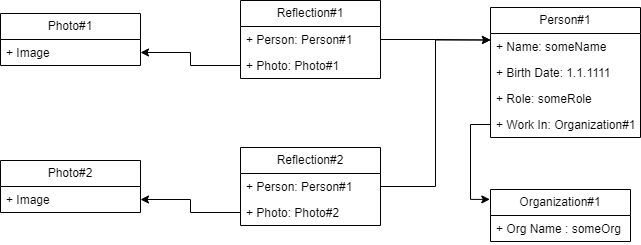
\includegraphics[width=0.6\textwidth]{_images/working_rdf.png}
    \caption{Запись, построенная по онтологии ЛШЮП}
    \label{fig:person_records}
\end{figure}

Используя следующее декларативное описание, которое описывает отображение любой записи, имеющий тип Person, использующиее визуальные элементы описанные выше вместе с многослойной привязкой

\begin{lstlisting}[language=XML]
<rdf:RDF
    xmlns:rdf="http://www.w3.org/1999/02/22-rdf-syntax-ns#"
    xmlns:sde="http://sde.org/type-vis-syntax-ns#">
<sde:VisualDescription rdf:type="Person">
<sde:Stack>
    <sde:ImageBox sde:Binding="!_->Reflection->Photo->Image"/>
    <sde:PropField sde:Name="Full Name" sde:Binding="Name"/>
    <sde:PropField sde:Name="Birthday" sde:Binding="Birth Date"/>
    <sde:PropField sde:Name="Role"/>
    <sde:ObjField  sde:Name="Work In" sde:ByName="Org Name"/>
<sde:Stack>
<sde:VisualDescription/>
\end{lstlisting}

После того, как мы получили требуемую запись, а также те, по которым мы переходим через привязки данных, мы получаем следующее визуальное представление записи (рис. \ref{fig:rdf_vis_result})

\begin{figure}
    \centering
    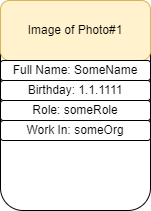
\includegraphics[width=0.2\textwidth]{_images/rdf_vis_result.png}
    \caption{Представление записи Person\#1}
    \label{fig:rdf_vis_result}
\end{figure}

\subsection{Выводы по 2 главе}
В этой главе были разобраны основные технологии и инструменты, применяемые в этой работе. Были рассмотрены различные модули клиентского приложения для работы с RDF данными. Были показаны модели данных, применяемые в данной работе. Также указана спецификация для создания собственных визуальных элементов.

\pagebreak
%======Конец Архитектура и алгоритмы=======================================================

%======Программная реализация==============================================================
\begin{center}
    {\section{Программная реализация}}
\end{center}

\subsection{Клиентская часть приложения}
\qquad Клиентская часть приложения использует модульную архитектуру, что позволяет создать определенный в рамках конкретного модуля контекст исполнения. Также используя механизм внедрения зависимостей, реализуемый с помощью DI Контейнера[18], и навигацию по различным модальным окнам, разработка в некоторых местах упрощается.

\subsubsection{Модули}
\qquad Приложение поделено на следующие модули:

\begin{enumerate}
    \item Node Editor (прил. 1) - модуль, позволяющий редактировать запись, то есть изменять, добавлять и удалять ссылки на другие записи, а также изменять значения литералов.
    \item Table View (прил. 2) - модуль, созданный для того, чтобы отображать записи в той форме, в которой они описаны в декларации визуального элемента. При отсутствии этой декларации строит DataGrid, в который отображаются записи без визуального сопровождения.
    \item Tree View (прил. 3) - модуль, нужный для того, чтобы отобразить связи между сущностями в виде древовидного представления. Так как он отображает только идентификаторы/имена сущностей, то он может довольно компактно отобразить большое количество связей. Также позволяет настраивать глубину возможных связей.
    \item Merge Resolver (прил. 4) - модуль, предоставляющий инструменты для решения конфликтов версии клиента и базы данных (гл. 3.3)
\end{enumerate}

\subsubsection{Semantic Web Context}
\qquad За хранение RDF данных и онтологии отвечают классы, выполняющие интерфейс ISemanticWebContext. Он содержит в себе методы, которые направлены на то, чтобы изменять топологию RDF графа, и методы для получения различной информации. На данный момент существуют 2 класса: SemanticWebInMemoryContext и SemanticWebDatabaseContext, которые соответственно работают с RDF данными, загруженные внутри приложения и с данными из удаленного источника, таких как база данных. Эта абстракция предоставляет возможность не задумываться об источнике данных во время написания логики работы с RDF графом.

\subsubsection{Ontology}
\qquad Класс, реализующий интерфейс IOntology, предоставляет удобное представление используемой в текущем контексте онтологии, как например свойства типа rdfs:domain и rdfs:range. С помощью этого становится известно какие значения хранит в себе сущность с данным типом, что позволяет строить визуальное представление в Table View.

\subsubsection{DI и Навигация}
Механизм навигации, который представлен в WPF Prism, дает нам лекго заменить Представление и Модель Представления в указанной области пользовательского интерфейса, или коротко говоря, поменять на другое модальное окно. Помимо этого у существует возможность передать данные, которые нужны для создания нового модального окна. Это заметно упрощает работу при переходе по ссылке к другой записи, так как для этого достаточно передать идентификатор сущности, к которой был совершен переход, и после, используя через механизм внедрения зависимостей ISemanticWebContext, можно сконструировать новое модальное окно.

\subsubsection{Построение визуального отображения записи}
\qquad Как можно заметить, формат XML имеет древовидную структуру. Чтобы упростить логику создания визуального отображения записи, можно воспользоваться шаблоном проектирования, который называется компоновщик ("Composite")[5]. Смысл его заключается в том, чтобы абстрагироваться от создания древовидных структур данных (рис. \ref{fig:composer_pattern}).

Главные элементы шаблона проектирования компоновщик следующие:
\begin{enumerate}
    \item Компонент - определяет общий интерфейс для простых и составных компонентов дерева.
    \item Лист — это простой компонент дерева, не имеющий ответвлений. Из-за того, что им некому больше передавать выполнение, классы листьев будут содержать большую часть полезного кода.
    \item Контейнер (или композит) — это составной компонент дерева. Он содержит набор дочерних компонентов, но ничего не знает об их типах. Это могут быть как простые компоненты-листья, так и другие компоненты-контейнеры. Но это не является проблемой, если все дочерние компоненты следуют единому интерфейсу. Методы контейнера переадресуют основную работу своим дочерним компонентам, хотя и могут добавлять что-то своё к результату.
\end{enumerate}

Если делить на листы и контейнеры компоненты визуализации записи, то получим следующее:
\begin{itemize}
    \item Контейнеры - sde:Stack, sde:List, sde:ListWrap, sde:Grid
    \item Листы - sde:ImageBox, sde:PropField, sde:ObjField
\end{itemize}

\begin{figure}[!ht]
    \centering
    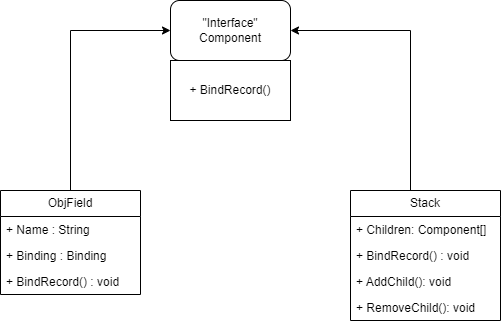
\includegraphics[width=0.5\textwidth]{_images/composer_arch.png}
    \caption{Шаблон проектирования компоновщик}
    \label{fig:composer_pattern}
\end{figure}

Данные компоненты соотвествуют интерфейсу IComponent. После создания компонента, мы привяжем Представление визуального компонента с моделью нашей записи, используя интерфейсный метод BindRecord().

\subsubsection{Алгоритм поиска записи по префиксу имени}
\qquad Для хранения имен индивидуальных сущностей, используются кэш имен. Кэш сохраняет значения для каждой записи в текущем RDF файле. По своей сути, кэш для имен именованных сущностей — это словарь, ключами которого являются имя или идентификатор индивидуальной сущности, в случае, если у нее нет имени, а значения - ссылки на запись, в которой хранится имя (или идентификатор) этой сущности.

Одним из запросов для кэша индивидуальных сущностей является запрос на получение ее записи по префиксу имени. Так как кэши сущностей хранят значение для всего RDF файла, то чтобы найти ее нам придется проходить через все имена и искать совпадающий префикс, так как мы не можем использовать префикс по той простой причине что его нет в словаре. При данном подходе такой запрос на запись занимает линейное время относительно количества записей в RDF файле. При большом количестве записей подобная ассимптотика может отрицательно сказываться на производительности.

Для ускорения ответа на запрос по получению записей по префиксу в работе было применено префиксное дерево[4] - древовидная структура данных, в вершинах которой находятся ссылки на другие вершины, а каждому ребру соответствует символ. Изначально в префиксном дереве находится стартовая вершина, к которой добавляются ребра и другие вершины. Пример префиксного дерева приведен на рис. \ref{fig:prefix_tree}. Благодаря префиксному дереву удобно и быстро искать все имена для заданного префикса, что позволяет нам реализовать авто-дополнение за довольно низкую ассимптотику.

\begin{figure}[!ht]
    \centering
    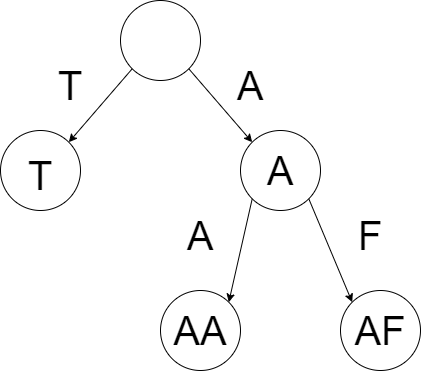
\includegraphics[width=0.5\textwidth]{_images/prefix_tree.png}
    \caption{Префиксное дерево}
    \label{fig:prefix_tree}
\end{figure}

Работает это по следующему принципу: при вводе нового символа в поисковой строке мы переходим по по ребру, у которого значение символа совпадает с введенным, после чего можно вывести в списке автодополнения все строковые идентификаторы, построенные от начальной вершины, далее все символы до вершины последнего введеного символа, и соответственно все оставшиеся символы до каждого из листа дерева, являющегося поддеревом от листа последнего введенного символа. В случае, если при введении нового символа не существуют ребер с этим символов, то это значит что такого идентификатора по крайней мере в кэшэ имен у клиента нет.

\pagebreak

\subsection{Архитектура серверной части приложения}
\qquad Архитектура серверной части приложения была построенна таким образом, чтобы была возможность работать с RDF данными из разных источников, таких как Neo4j или PolarDB[19] не нарушая при этом принцип инверсии зависимостей[18]. Таким образом, важным критерием является создание абстракции вокруг источника данных, приводящий эти данные к единому формату. Это позволяет в рамках одной кодовой базы для логики сервера предоставить клиентской части приложения унифицированный API для доступа к данным, находящихся на  абстрактном удаленном хранилище, что позволяет сократить время разработки новых адаптеров для данных (рис. \ref{fig:data_access}).

\begin{figure}[!ht]
    \centering
    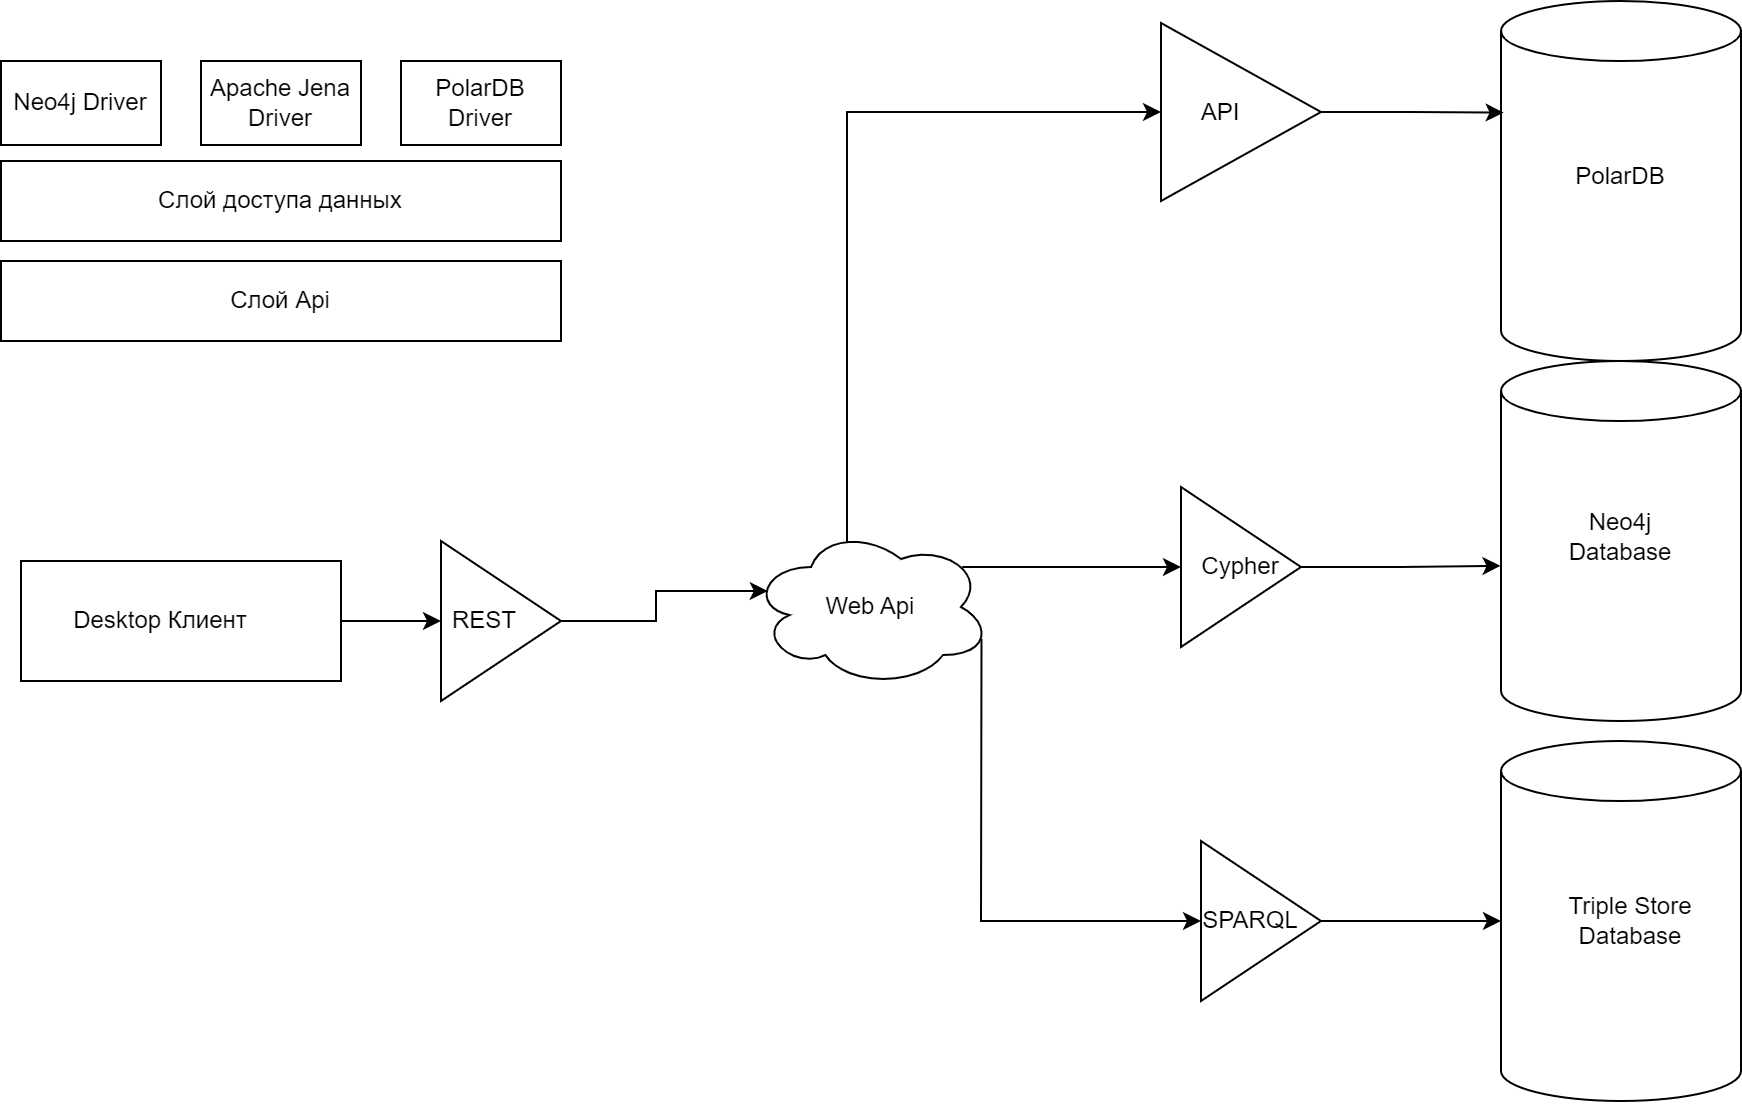
\includegraphics[width=0.7\textwidth]{_images/data_access.png}
    \caption{Доступ к данным}
    \label{fig:data_access}
\end{figure}

Можно заметить, что существует такой язык запросов как SparQL, который задумывался как способ обращения к источнику связанных данных, как например RDF. Но на данный момент не все базы данных связанных данных его поддерживают, а некоторые базы данных, как например Neo4j, его поддержку прекратили. В рамках данной работы реализован адаптер для графовой базы данных Neo4j и использована соответственно база данных Neo4j, так как на данном примере легко показать, что язык запросов SparQL нельзя считать средством, которое позволяет решить проблемы с абстрактным доступом к данным.

\subsubsection{Кэширование данных на стороне клиента}
\qquad Главной особенностью клиент-серверного приложения является то, что пользователь не хранит все данные, которые лежат на удаленном источнике. В противном случае, если клиент просто скачивает данные с сетевой части, клиент-серверное приложение просто превращается в клиентское. Главной идеей этой работы является то, что пользователь во время работы при обращении к нужной части удаленного ресурса динамически подкачивает его на клиентскую часть приложения. Это особенно выгодно смотрится в тех случаях, когда размер ресурса превышает количество доступной памяти на пользовательском устройстве, а также когда необходимо начать работать с источником данных как можно скорее. Чтобы реализовать механизм динамической подкачки данных была разработана следующая схема, представленная на рис. \ref{fig:remote_conn}.

\begin{figure}[!ht]
    \centering
    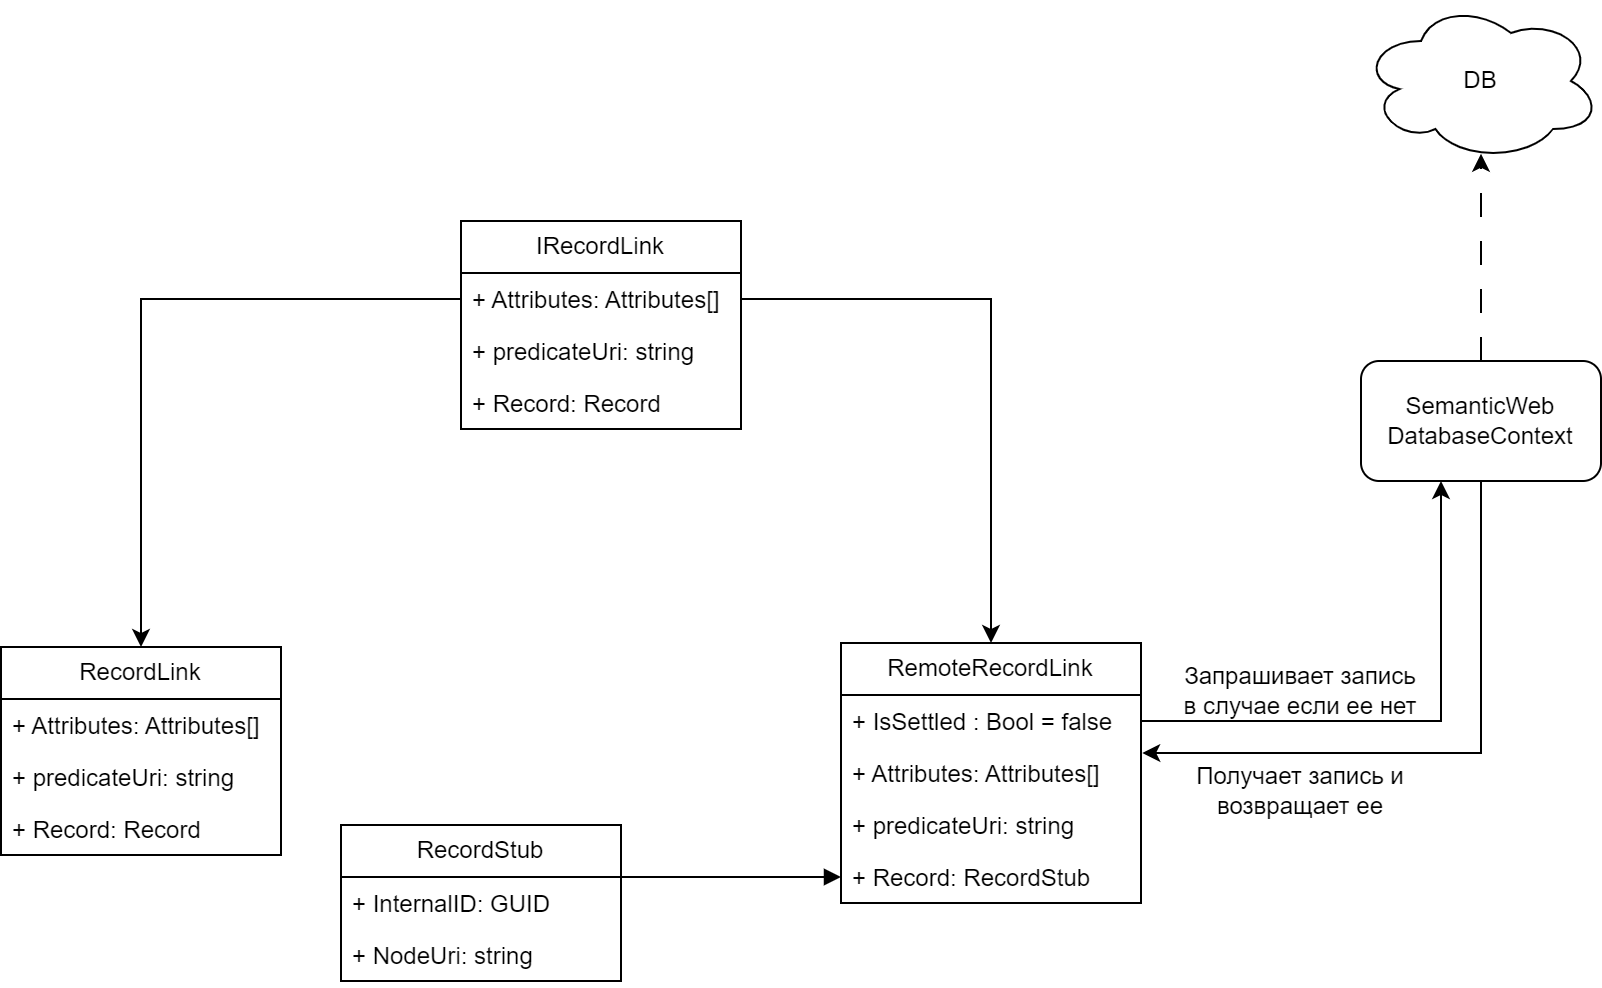
\includegraphics[width=0.5\textwidth]{_images/remote_conn.png}
    \caption{Механизм динамической подкачки}
    \label{fig:remote_conn}
\end{figure}

Чтобы абстрагироваться от источника данных, используется интерфейс IRecordLink. Если выбран режим работы, когда все данные загружаются на прямую в память компьютера, используется RecordLink. Если мы работаем с удаленным источником данных, то используется RemoteRecordLink. Каждый раз когда мы обращаемся к полю RemoteRecordLink.Record, мы проверяем, храним ли мы реальную ссылку на запись или нет. В противном случае мы обращаемся к сервису SemanticWebDatabaseContext, которая в свою очередь обращается к базе данных, из которой мы получаем запись, которой до этого у нас не было. При этом мы также кэшируем в память полученную запись, чтобы в дальнейшем не тратить I/O ресурсы на получение записи, которую уже была когда-то получена.

\subsubsection{Взаимодействие клиента с сервером}
\qquad Для этого в данной работе был создано свое собственное API для обращению к серверу, которое не предполагает той гибкости, что SparQL, но тем не менее удовлетворяет всем формальным требованиям клиентской части приложения.

Сервис для получения данных выполнен в рамках архитектурного шаблона REST (REpresentational State Transfer)[20]. Ключевым ресурсом, с которым веб сервис работает, в контексте GET запросов является Record, представленный в клиентской части приложения.

Следующим важным элементом в рамках клиент-серверного сообщения являются команды на изменение Record в базе данных. С помощью команд достигается уменьшение размера сообщения между клиентом и сервером, так как в таком случае мы передаем только одно из измененных значений Record:

\begin{verbatim}entity/change_dt_prop{id1}{prop_name}{new_value} \end{verbatim}

Важным отличием данного подхода является то, что обеспечивается более прозрачный API, а также появляется возможность перенести часть доменной логики из клиента в серверную часть приложения, так как задачей клиента является обеспечить представление данных[21].

В качестве формата для сообщения между сервером и клиентом был выбран формат JSON, из-за его простоты относительно бинарной сериализацией, а также легкостью относительно XML формата. Для описания методов API была спроектирована спецификации OpenApi 3.0[22].

\subsubsection{REST запросы}
На текущий момент для обращению к серверу существуют следующие команды:

\begin{enumerate}
    \item \begin{verbatim} entity/add_node/{addedNodeUri}/{nodeType} \end{verbatim}
          - добавить узел с идентификатором addedNodeUri и типом nodeType
    \item \begin{verbatim} entity/delete_node/{deletedNodeUri}\end{verbatim}
          - удалить узел с идентификатором deletedNodeUri
    \item \begin{verbatim} entity/add_property/{nodeUri}/{propertyName}/{propertyType}\end{verbatim}
          - добавить к узлу с идентификатором nodeUri свойство с именем propertyName объектного или символьного типа
    \item \begin{verbatim} entity/change_obj_property/{nodeUri}/{changedPropName}/{changedNodeUri} \end{verbatim}
          - изменить объектное свойство с именем changedPropName у узла с идентификатором nodeUri на объект с идентификатором changedNodeUri
    \item \begin{verbatim}entity/change_obj_property/{nodeUri}/{changedPropName}/{changedLiteral} 
\end{verbatim}
          - изменить символьное свойство с именем changedPropName у узла с идентификатором nodeUri на символ changedLiteral
\end{enumerate}

При редактировании узлов на клиенте они сначала сохраняются в локальных изменениях, выраженные через команды выше, и в нужный момент клиент отправляет все эти изменения одним запросом, чтобы таким образом совершить изменения в базе данных в рамках одной транзакции, что в свою очередь позволяет сократить накладные расходы на взаимодействие с базой данных.

\begin{verbatim}     data/push_changes/{clientVersion} \end{verbatim}
\qquad - где в теле запроса представлены все совершенные изменения.

Для получения данных существуют следующие REST запросы:

\begin{enumerate}
    \item \begin{verbatim} entity/get_node/{NodeId}/{clientVersion} \end{verbatim}
          - получить узел с внутренним идентификатором NodeId, соответствующий версии clientVersion в виде JSON представления
    \item \begin{verbatim} data/get_changes/{clientVersion} \end{verbatim}
          - получить все изменения относительно версии клиента clientVersion
\end{enumerate}

\subsection{Обеспечение конкурентного доступа к данным}
Так как с приложением что с приложением будет работать больше чем один человек, то существует проблема, связанная с тем, что изменения, произведенные на стороне клиента, могут конфликтовать с изменениями, совершенными на стороне другого клиента в том случае, когда пользователи работают над одним и тем же RDF источником данных одновременно. Соответственно, в рамках работы стоит задача, позволяющая разрешить данные конфликты изменений.

\subsubsection{Система контроля версиями}
\qquad В качестве решения проблемы одновременного редактирования источника данных были рассмотрены различные методы, как например long-polling[26] или WebSockets[27]. Их недостатком является то, что они требуют для работы постоянного подключения к сети Интернет и больше предназначены для работы с приложением в реальном времени, что в данной работе не требуется. Помимо этого возникает проблема взаимодействия с клиентом, когда пользователя каждый раз будут отвлекать оповещения сервера о том, что произошел конфликт изменений.

Другим возможным решением, которым была решена задача, является использование концепции системы контроля версий (англ. Version Control System, сокр. VCS)[28]. Ее использование обусловленно тем, что все запросы на изменения данных являются относительными: вместо перезаписывания всей записи, отправляется запрос на изменение только конкретного участка записи, что является одной из идеей, заложенной в концепции VCS.

В работе была реализована базовая система контроля версий, которая на данный момент поддерживает следующие операции:

\begin{enumerate}
    \item Зафиксировать все изменения в источник (push в терминах VCS)
    \item Принять изменения из источника (pull в терминах VCS). Если есть изменения на стороне базы данных, то происходит обновление кэша клиента, и в случае конфликта предоставляется средство для слияния изменений клиента и базы данных (merge в терминах VCS)
\end{enumerate}

\subsubsection{Отправка изменений на сервер}
\qquad Для существования системы контроля версий на стороне сервера, помимо самой RDF базы данных (RDF Database), в которой хранится текущее состояние, существует вторая база данных (Commit Database), которая хранит в себе все изменения состояний. Помимо самих изменений, в ней еще находится счетчик версии RDF базы данных, за счет которого осуществляется корректное версионирование состояния. В качестве Commit Database было выбрано решение MongoDB[29], так как она позволяет главным образом хранить разнородные данные, чем и являются в своем виде изменения.

Передача и фиксация изменений может иметь два возможных исхода: успешная фиксация изменений или конфликт между состояниями данных клиента и RDF базы данных.

В первом случае, если версии данных клиента и базы данных совпадают, то происходит фиксация изменений в RDF базе данных, а также добавляются изменения в Commit Database. Клиенту приходит ответ, что запись изменений произошла успешно.

\begin{figure}[!ht]
    \centering
    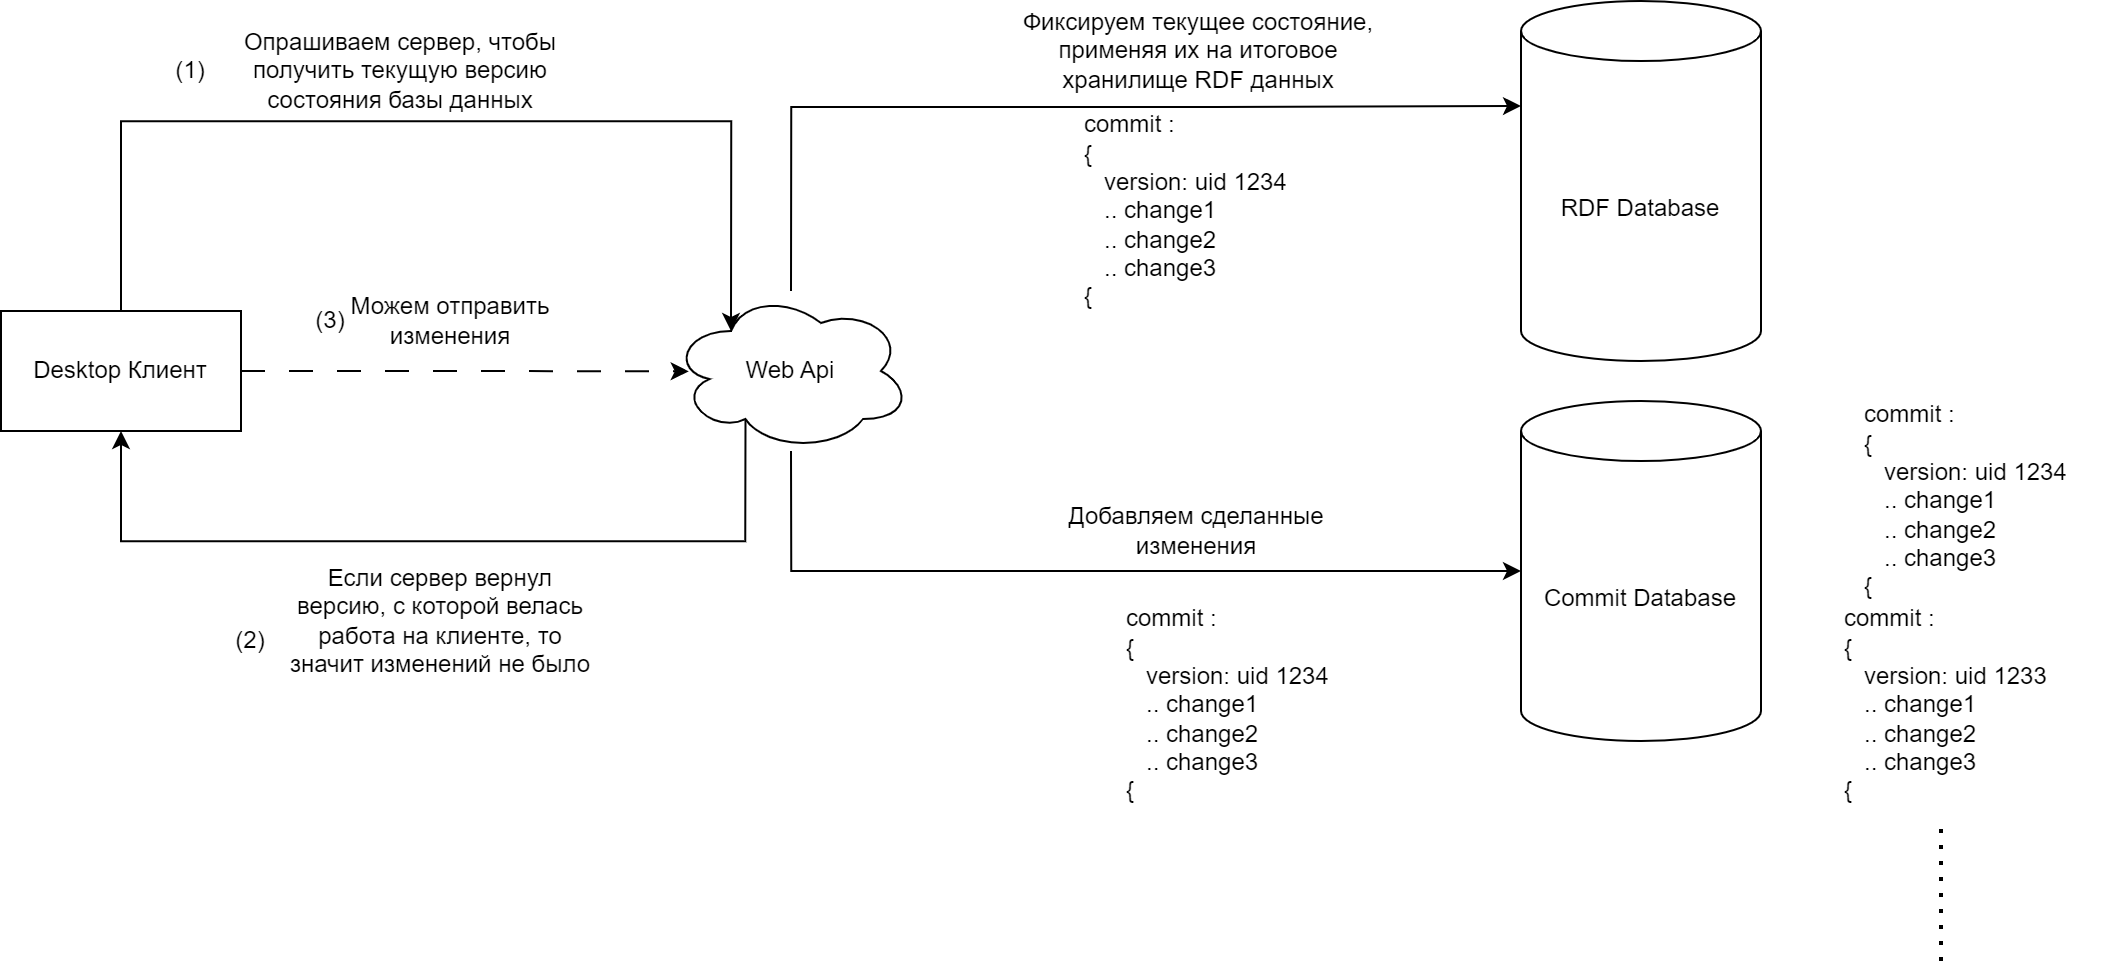
\includegraphics[width=0.7\textwidth]{_images/if_merge_success.png}
    \caption{Фиксация изменений при отсутствии конфликтов}
    \label{fig:if_merge_success}
\end{figure}

В втором случае, если версия данных у клиента оказывается меньше чем версия базы данных, то это указывает на то, что может произойти конфликт. Чтобы проверить наличие конфликта между данными клиента и базы данных, мы запрашиваем все изменения из Commit Database, начиная от версии клиента и заканчивая последним изменением на стороне сервера.

\begin{figure}[!ht]
    \centering
    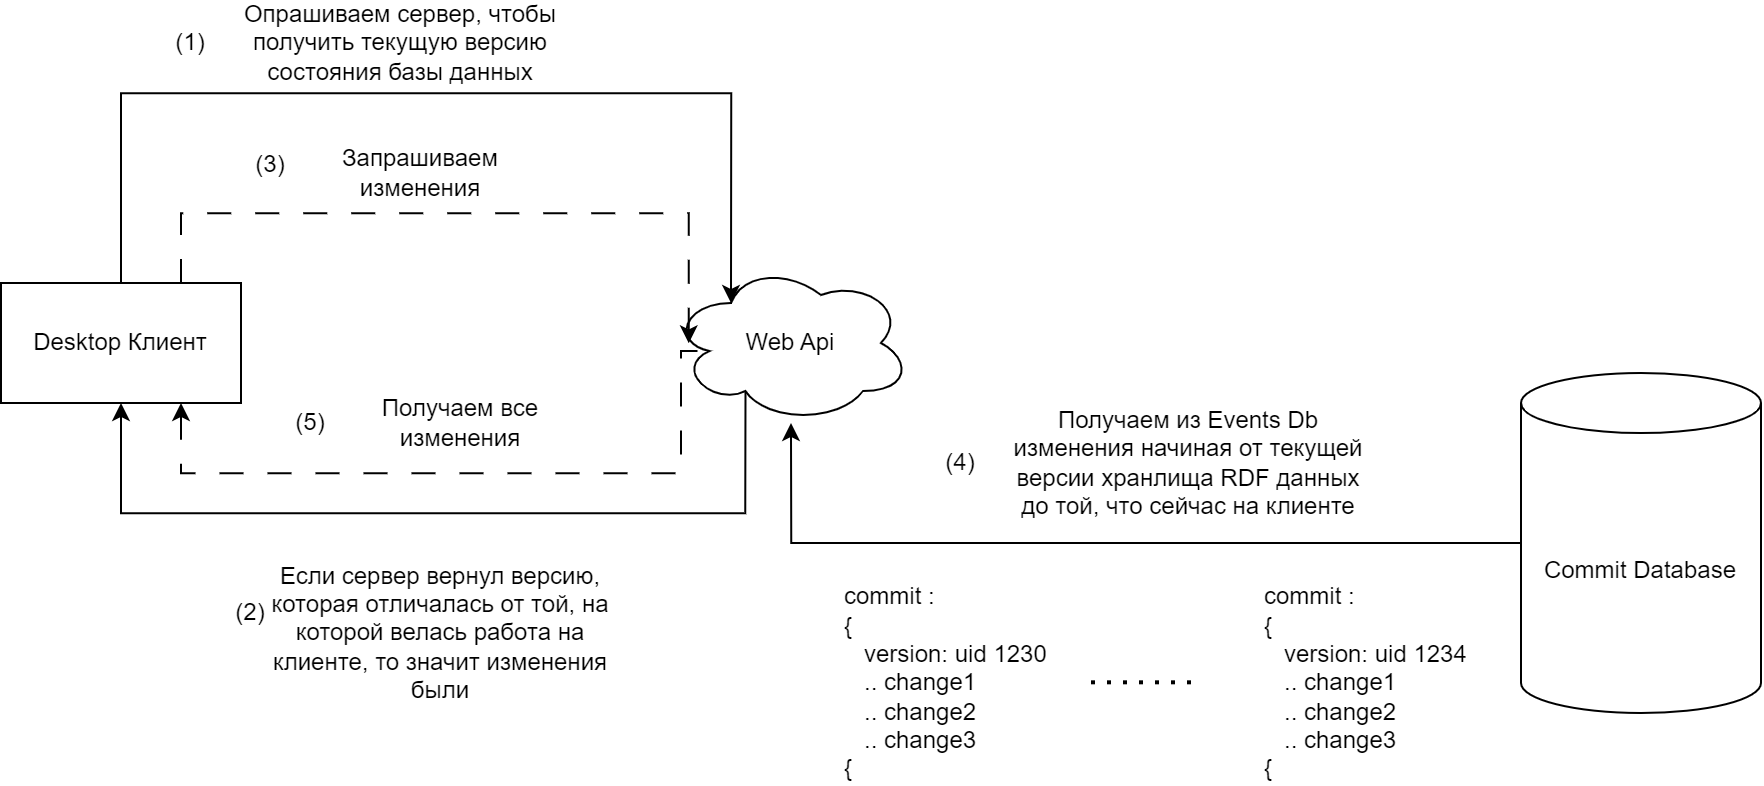
\includegraphics[width=0.7\textwidth]{_images/if_merge_failure.png}
    \caption{Фиксация изменений при наличии конфликтов}
    \label{fig:if_merge_failure}
\end{figure}

\subsubsection{Проблема подкачки узлов при несоответстующих версиях}
\qquad При работе на определенной версии базы данных существует проблема, связанная с тем, что подкачка узла по ссылке может осуществляться уже из обновленного источника. Соответственно, возникают следующие проблемы (рис. \ref{fig:noncorrect_node_pump}):

\begin{enumerate}
    \item Символьные и объектные свойства могут иметь разные значение или ссылаться на различные узлы соответственно.
    \item При удалении в новой версии узла, на который уже не существует ссылка, в версии клиента эта ссылка продолжает указывать на существующий узел. Соответственно, при подкачке этого узла в старой версии мы его не сможем получить по его ресурсному идентификатору.
    \item Переименование узла приводит также приводит к проблеме выше.
\end{enumerate}

\begin{figure}[!ht]
    \centering
    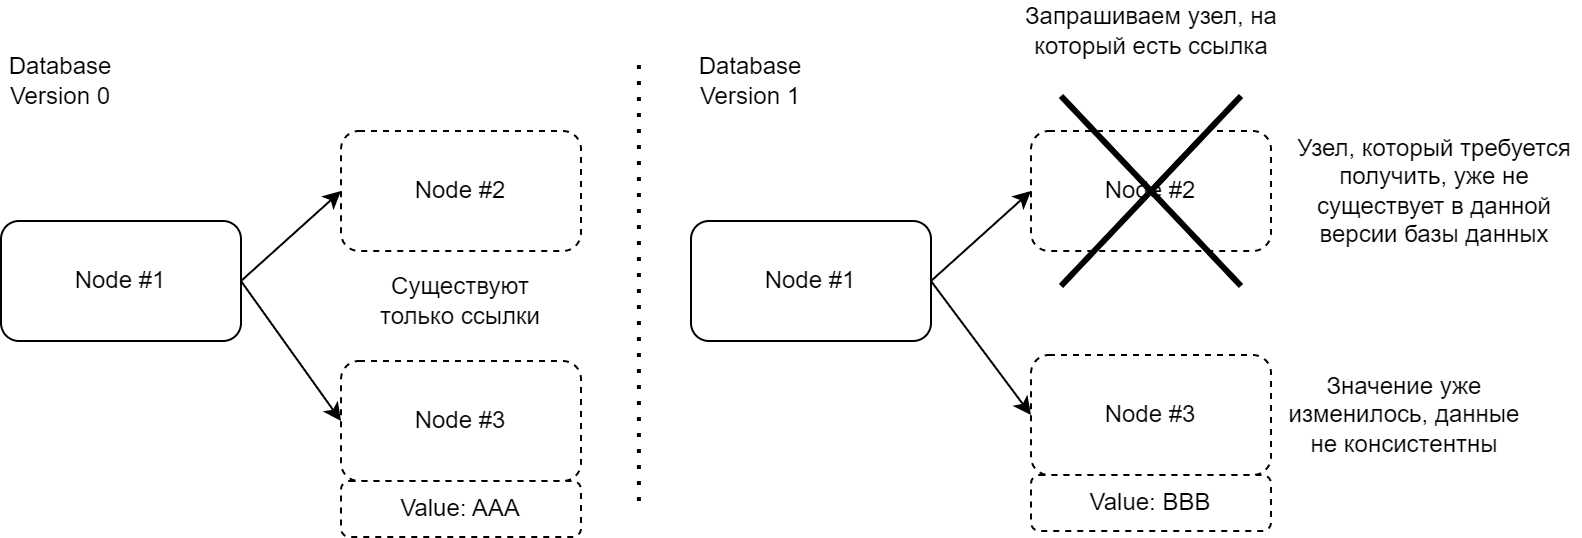
\includegraphics[width=0.7\textwidth]{_images/bad_node_pooling.png}
    \caption{Некорректная подкачка узлов}
    \label{fig:noncorrect_node_pump}
\end{figure}

Для решение данной проблемы были сделаны следующие модификации: добавление истории изменения текущего узла в сам узел на стороне базы данных, а также присвоение каждому узлу внутреннего идентификатора (InternalID). Первая модификация решает проблему версионирования значений свойств, так как вместе с запросом на получение узла указывается ожидаемая версия, после чего можно откатить все изменения до данной версии, а вторая позволяет сохранить связи при удалении или переименованию узлов в текущей версии базы данных.

\pagebreak

\subsubsection{Синхронизация одновременных запросов на изменение}
\qquad Существует вероятность, что два или более пользователя могут отправить запросы на изменения данных, при этом имея на своей стороне данные последней версии. В таком случае может произойти такая ситуация, что уже в самой базе данных возникает конфликт, так как применяются изменения из обоих запросов, которые могут содержать конфликты, не говоря уже о том, что в Commit Database оказываются изменения с двумя одинаковыми номерами версий, таким образом нарушая ее главный инвариант - линейный рост номеров версий, приводя ее тем самым в невалидное состояние.

Стоит заметить, что повышение версии базы данных сразу при получении запроса на изменение имеет следующую проблему: если применение изменений первого клиента завершились ошибкой, то у следующего клиента тем временем будет тем не менее конфликт изменений, так как версии данных клиента и базы данных уже отличаются, но при этом с точки зрения механизма работы системы контроля версии изменения следующего клиента могут быть зафиксированны в базе данных (при условии что они сами являются валидными).

Для решения этой проблемы, не имея при этом недостаток выше, можно воспользоваться средствами синхронизации. Для этого на стороне сервера используется глобальный бинарный асинхронный семафор[30]. Механизм работы сервера при одновременых запросах представлен на (рис. \ref{fig:concurrent})

\begin{figure}[!ht]
    \centering
    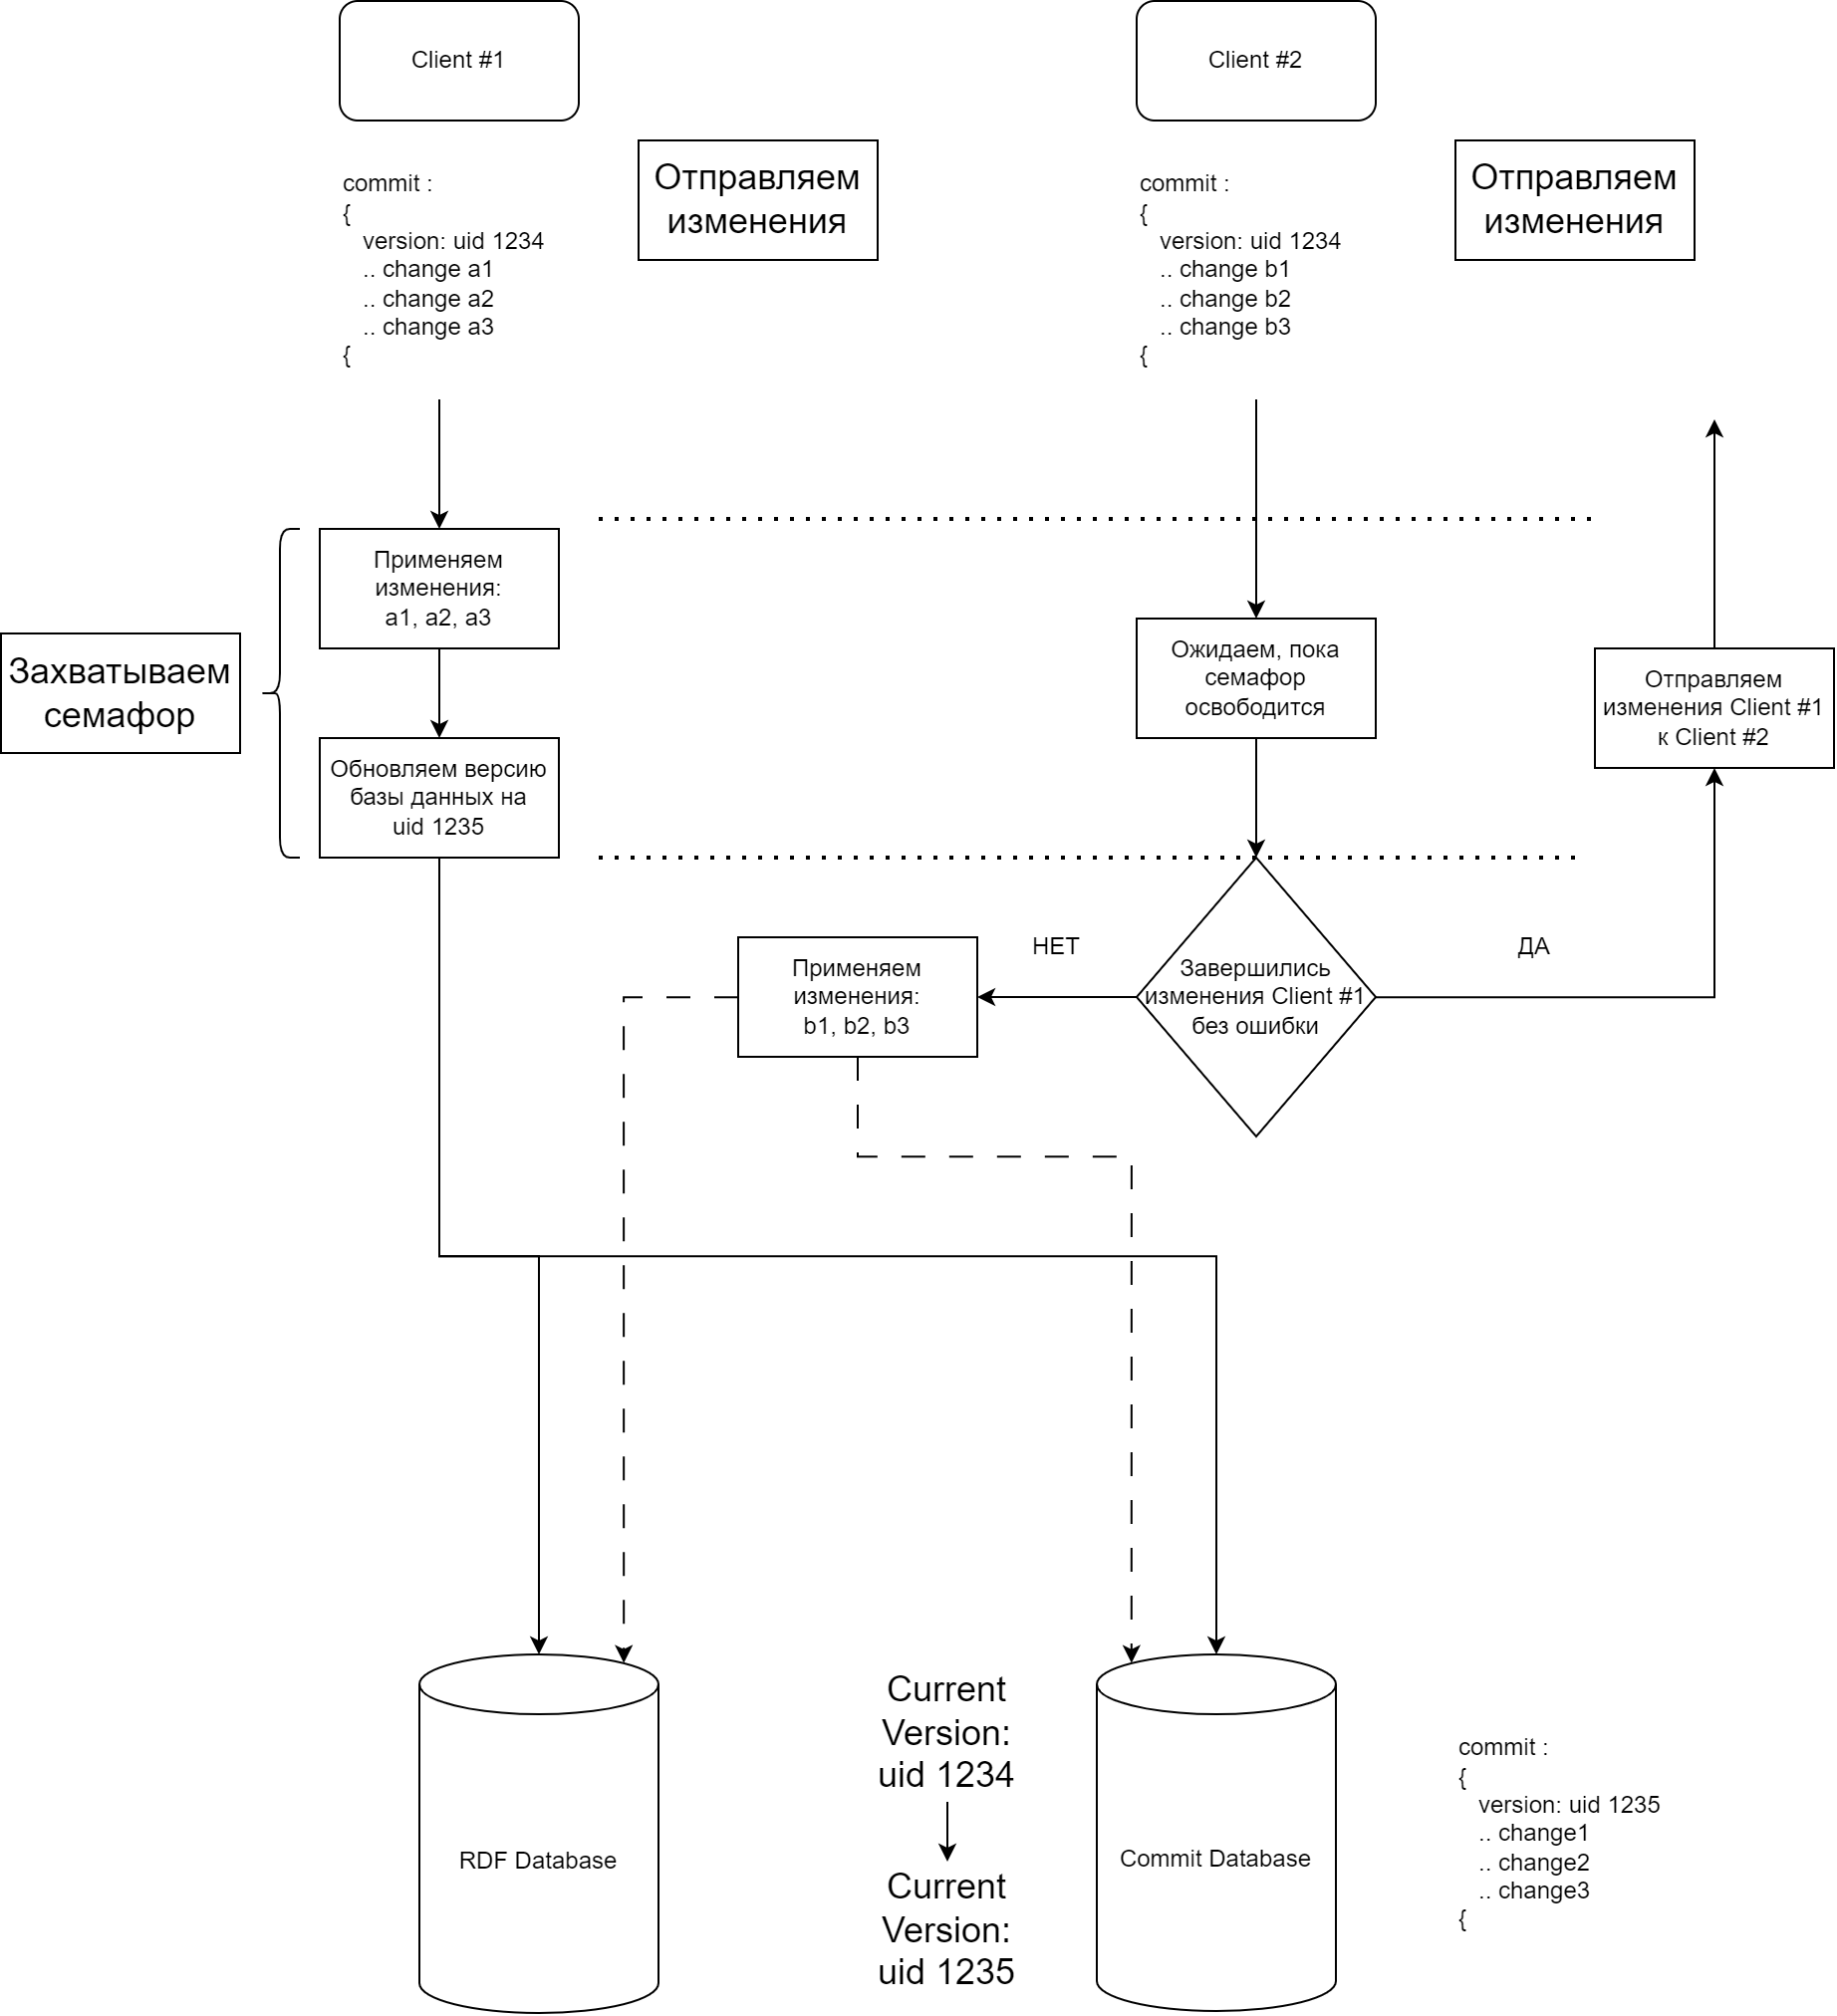
\includegraphics[width=0.7\textwidth]{_images/concurrent_push_good.png}
    \caption{Корректная подкачка узлов}
    \label{fig:concurrent}
\end{figure}

\pagebreak

\subsection{Слияние изменений}
\qquad В системах контроля версий существует инструмент, который позволяет разрешать конфликты одновременных версий. В работе этот инструмент реализован в рамках модуля Merge Resolver, который позволяет принимать или переписывать уже сделанные измененения, в том числе в частичном порядке.

Существуют следующие виды конфликтов:

\begin{enumerate}
    \item Различные значения символьных свойств
    \item Различные ссылки объектных свойств
    \item Удаление узла, на котором были редактированы свойства
\end{enumerate}

При фиксации разрешенных конфликтов отправляется запрос на изменение данных с версией, которая больше на единицу чем та, которая содержала конфликты. В случае выхода из режима слияния изменений, версия клиента и данные остаются теми же, что были до этого.

\subsection{Выводы по третьей главе}
\qquad В этой главе были разобраны основные составляющие клиентской и серверной части приложения, а также был показан механизм реализации построения визуального элемента. Также были рассмотрены и выбраны протоколы сообщений между клиентом и сервером, среди них был выбран наиболее подходящий вариант. Были решены проблемы, связанные с проблемами изменения данных при работе множества пользователей.

\pagebreak
%======Конец Программной реализации========================================================

\sectionfont{\centering}
%======Заключение==========================================================================
\begin{center}
    {\anonsection{Заключение}}
\end{center}

Можно подвести итоги проделанной работы. В рамках работы над приложением "Semantic Data Editor" реализована функциональность для интерактивного и интуитивного отображения данных в формате RDF. Для редактирования и отображения данных были созданны следующие компоненты: Table View, Node Editor View. Наличие этих компонентов позволяет выбрать оптимальный режим работы: для анализа текущей записи и всех ее соседей удобно использовать Table View, если же нужно перейти в режим редактирования записи достаточно найти ее через поиск или перейти по ссылке в текущей записи. Также в рамках кооперативной работы пользователей была разработана инфраструктура и инструменты. Для комфортной работы с RDF данными существует меню настроек и специальный синтаксис, благодаря которым можно редактировать различные параметры для отображения и редактирования, а также различные дополнения в схеме онтологии.\par

В данной работе была также представлена серверная часть приложения, которая позволяет работать с большими данными на любом устройством и не хранить большой объем информации на своем физическом носителе. При этом у пользователя все также остается возможность использовать локальную базу данных, либо использовать In-Memory хранилище данных.\par

В рамках развития приложения планируется добавлять больше тестов, следить за репозиторием приложения на предмет багов, которые могут заводить пользователи приложения, а также проводить рефакторинг для улучшения производительности и более гибкой архитектуры приложения.\par

Проект «Semantic Data Editor» является open-source проектом, распространяемым под MIT[31] лицензией, и опубликован в удаленном репозитории GitHub[32].

\pagebreak
%======Конец Заключения====================================================================

%======Литература==========================================================================
\begin{center}
    {\anonsection{Литература}}
\end{center}

\begin{flushleft}
    [1] Allemang D, Hendler. J. Semantic Web for working ontologysts 2nd Edition. Massachusetts, Morgan Kaufmann Publishers, 2011. 349 с.

    [2] Auer S., Lehmann J. Creating Knowledge out of Interlinked Data // Semantic Web Journal - Январь 2010. 97-104 с.

    [3] RDF 1.1 Concepts and Abstract Syntax [Электронный ресурс] -2014. -Режим доступа: https://www.w3.org/TR/rdf11-concepts/

    [4] RDF 1.1 XML Syntax [Электронный ресурс] -2014. -Режим доступа: https://www.w3.org/TR/rdf-syntax-grammar/

    [5] Notation3 (N3): A readable RDF syntax [Электронный ресурс] -2014. -Режим доступа: https://www.w3.org/TeamSubmission/n3/

    [6] RDF 1.1 Turtle [Электронный ресурс] -2014. -Режим доступа: https://www.w3.org/TR/turtle/

    [7] RDF Schema 1.1 [Электронный ресурс] -2014. -Режим доступа: https://www.w3.org/TR/rdf-schema/

    [8] OWL Web Ontology Language Overview [Электронный ресурс] -2004. -Режим доступа: https://www.w3.org/TR/owl-features/

    [9] Extensible Markup Language (XML) 1.0 (Fifth Edition) [Электронный ресурс] -2009. -Режим доступа: https://www.w3.org/TR/xml/

    [10] Introducing JSON [Электронный ресурс] -1999. -Режим доступа: https://www.json.org/json-en.html

    [11] Medical Subject Headings [Электронный ресурс] -Режим доступа: https://www.nlm.nih.gov/mesh/meshhome.html

    [12] WPF [Электронный ресурс] -Режим доступа: https://learn.microsoft.com/ru-ru/visualstudio/get-started/csharp/tutorial-wpf?view=vs-2022

    [13] MVVM [Электронный ресурс] -Режим доступа: https://learn.microsoft.com/ru-ru/dotnet/architecture/maui/mvvm

    [14] MVC [Электронный ресурс] -Режим доступа: https://developer.mozilla.org/en-US/docs/Glossary/MVC

    [15] MVP [Электронный ресурс] -Режим доступа: https://learn.microsoft.com/en-us/archive/msdn-magazine/2006/august/design-patterns-model-view-presenter

    [16] Prism Library [Электронный ресурс] -Режим доступа: https://prismlibrary.com/docs/

    [17] Общие сведения об ASP.NET Core [Электронный ресурс] -Режим доступа: https://learn.microsoft.com/ru-ru/aspnet/core/introduction-to-aspnet-core?view=aspnetcore-8.0

    [18] Martin R.C. Clean Code: A Handbook of Agile Software Craftsmanship. London, Pearson, 2008. 464 с.

    [19] Марчук А.Г. Последовательность как абстракция структурированного построения баз данных / Марчук А. Г. // System Informatics (Системная информатика), No. 18 (2021)

    [20] Fielding R.-T. Representational State Transfer [Электронный ресурс] - Режим доступа:  https://ics.uci.edu/~fielding/pubs/dissertation/rest\_arch\_style.htm

    [21] Young G. CQRS and Event Sourcing [Электронный ресурс] -Режим доступа: https://cqrs.wordpress.com/wp\_content/uploads/2010/11/cqrs\_documents.pdf

    [22] OpenApi [Электронный ресурс] -Режим доступа: https://www.openapis.org/

    [23] MacDonald M. Pro WPF 4.5 in C\#: Windows Presentation Foundation in .NET. New York, Apress, 2012. 1111 с.

    [24] Skiena S.S. The Algorithm Design Manual 2nd Edition. New York, Springer, 2010. 748 с.

    [25] Gamma E., Helm R., Johnson R., Vlissides J. Design Patterns: Elements of Reusable Object-Oriented Software 1st Edition. New York, Addison-Wesley Professional, 1994. 416 с.

    [26] HTTP Long Polling [Электронный ресурс] -Режим доступа: https://ably.com/topic/long-polling

    [27] WebSocket: что это, когда следует использовать и какие преимущества дает [Электронный ресурс] -Режим доступа: https://cloud.vk.com/blog/websocket-kogda-sleduet-ispolzovat-i-preimushhestva

    [28] Введение - О системе контроля версий [Электронный ресурс] -Режим доступа: https://git-scm.com/book/ru/v2/ВВедение-О-системе-контроля-версий

    [29] MongoDB Manual - [Электронный ресурс] -Режим доступа: https://www.mongodb.com/docs/manual/

    [30] Richter J. CLR via \verb|C#| 4th Edition. London, Microsoft Press, 2012. 896 с.

    [31] Лицензия MIT - [Электронный ресурс] -Режим доступа: \verb|https://ru.wikipedia.org/wiki/Лицензия_MIT|

    [32] GitHub Репозиторий - [Электронный ресурс] -Режим доступа: \verb| https://github.com/Krazerleo/SemanticWeb_DataBase|

\end{flushleft}

\pagebreak

\begin{center}
    {\anonsection{Приложение}}
\end{center}

\begin{figure}[!ht]
    \centering
    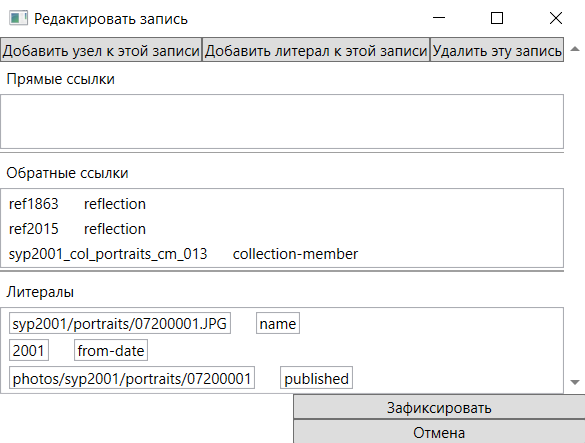
\includegraphics[width=0.6\textwidth]{_images/edit_window.png}
    \caption*{Прил. 1: Окно редактирования записи}
    \label{app:edit_node_view}
\end{figure}

\begin{figure}[!ht]
    \centering
    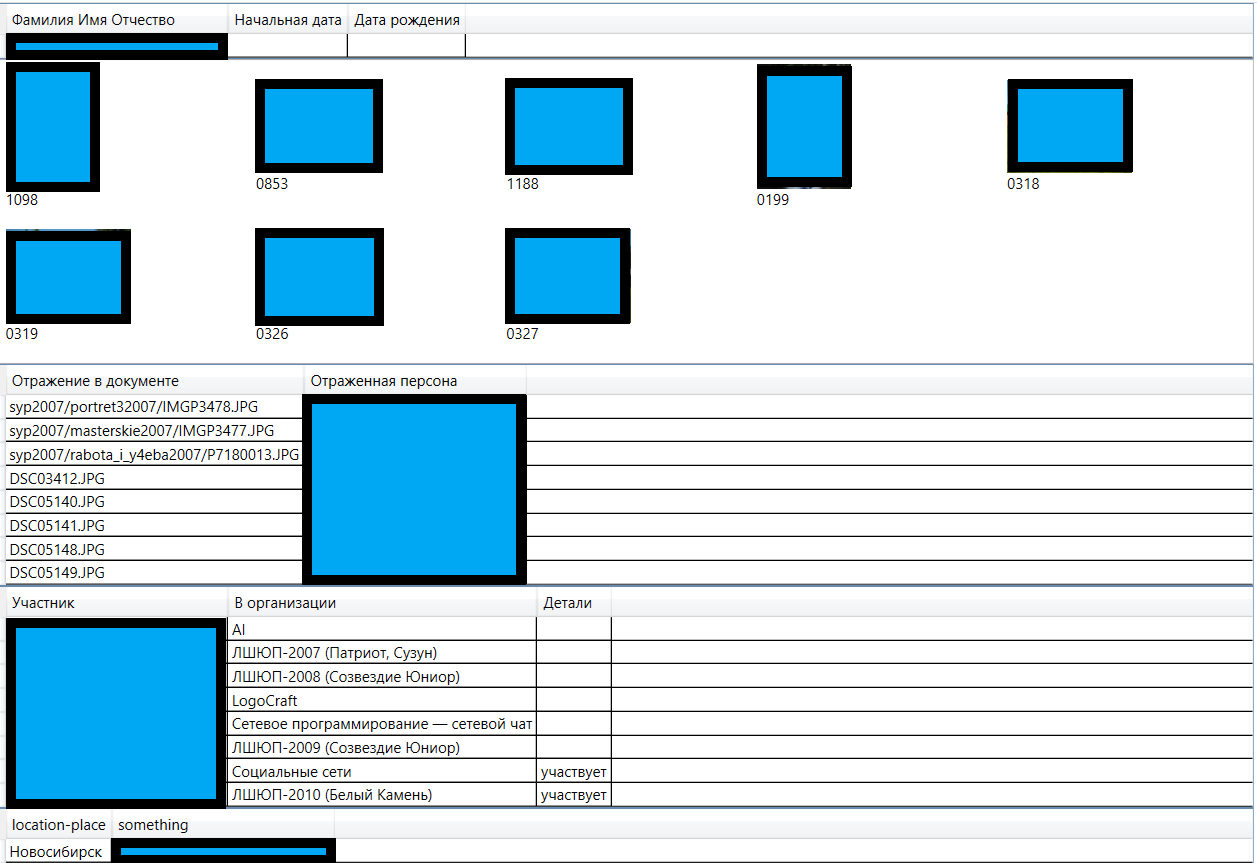
\includegraphics[width=0.7\textwidth]{_images/table_view.png}
    \caption*{Прил. 2: Окно табличного представления}
    \label{app:table_view}
\end{figure}

\begin{figure}
    \centering
    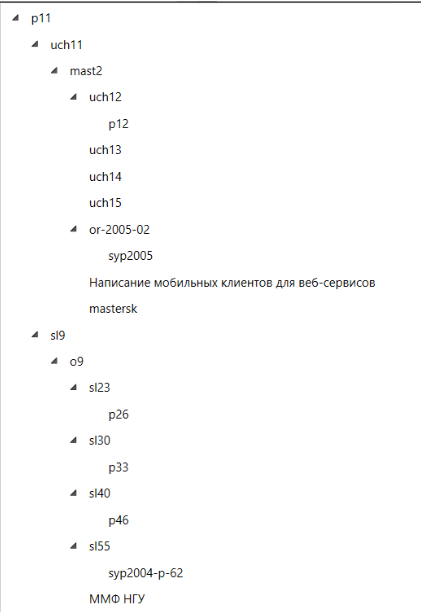
\includegraphics[width=0.6\textwidth]{_images/tree_view.png}
    \caption*{Прил. 3: Окно древовидного представления}
    \label{app:tree_view}
\end{figure}

\begin{figure}
    \centering
    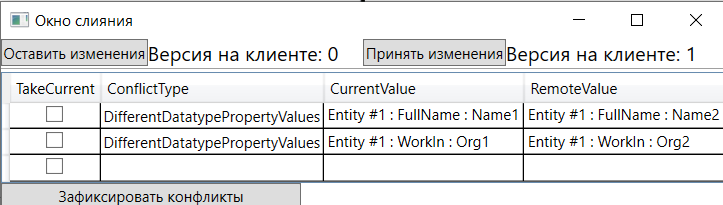
\includegraphics[width=0.8\textwidth]{_images/merge_tool.png}
    \caption*{Прил. 4: Средство слияния изменений}
    \label{app:merge_tool}
\end{figure}
\pagebreak
%======Конец Литературы====================================================================
\end{document}